% WACV 2025 Paper Template
% based on the WACV 2024 template, which is
% based on the CVPR 2023 template (https://media.icml.cc/Conferences/CVPR2023/cvpr2023-author_kit-v1_1-1.zip) with 2-track changes from the WACV 2023 template (https://github.com/wacv-pcs/WACV-2023-Author-Kit)
% based on the CVPR template provided by Ming-Ming Cheng (https://github.com/MCG-NKU/CVPR_Template)
% modified and extended by Stefan Roth (stefan.roth@NOSPAMtu-darmstadt.de)

\documentclass[10pt,twocolumn,letterpaper]{article}

%%%%%%%%% PAPER TYPE  - PLEASE UPDATE FOR FINAL VERSION
%\usepackage[review,algorithms]{wacv}% To produce the REVIEW version for the algorithms track
%\usepackage[review,applications]{wacv}% To produce the REVIEW version for the applications track
\usepackage{wacv}  % To produce the CAMERA-READY version
%\usepackage[pagenumbers]{wacv} % To force page numbers, e.g. for an arXiv version

% Include other packages here, before hyperref.
\usepackage{graphicx}
\usepackage{amsmath}
\usepackage{amssymb}
\usepackage{booktabs}
\usepackage{multirow}
\usepackage{algorithm}
\usepackage{algorithmicx} % <===========================================
\usepackage{algpseudocode} % <==========================================
\usepackage{setspace}
\usepackage{bm}
\usepackage{tikz}
\usepackage{array}
\usepackage{makecell}
\usepackage{diagbox}
% \geometry{margin=0.8in}
\usepackage{float}

\usepackage{tocloft}
% \setlength{\cftsecnumwidth}{1.7em}
% \setlength{\cftsubsecnumwidth}{2.5em}

\newcommand{\ballnumber}[1]{\tikz[baseline=(myanchor.base)] \node[circle,fill=.,inner sep=1pt] (myanchor) {\color{-.}\bfseries\footnotesize #1};}
% It is strongly recommended to use hyperref, especially for the review version.
% hyperref with option pagebackref eases the reviewers' job.
% Please disable hyperref *only* if you encounter grave issues, e.g. with the
% file validation for the camera-ready version.
%
% If you comment hyperref and then uncomment it, you should delete
% ReviewTempalte.aux before re-running LaTeX.
% (Or just hit 'q' on the first LaTeX run, let it finish, and you
%  should be clear).

% begin vertical rule patch for algorithmicx (http://tex.stackexchange.com/questions/144840/vertical-loop-block-lines-in-algorithmicx-with-noend-option)
% note that some of the packages above are also needed
\usepackage{tikz}
\usetikzlibrary{tikzmark}
\usepackage{pifont}% http://ctan.org/pkg/pifont
\newcommand{\cmark}{\ding{51}}%
\newcommand{\xmark}{\ding{55}}%
\usetikzlibrary{calc}
\errorcontextlines\maxdimen
\newcommand{\ALGtikzmarkcolor}{black}% customise this, if you want
\newcommand{\ALGtikzmarkextraindent}{4pt}% customise this, if you want
\newcommand{\ALGtikzmarkverticaloffsetstart}{-.5ex}% customise this, if you want
\newcommand{\ALGtikzmarkverticaloffsetend}{-.5ex}% customise this, if you want
\makeatletter
\newcounter{ALG@tikzmark@tempcnta}

\newcommand\ALG@tikzmark@start{%
\global\let\ALG@tikzmark@last\ALG@tikzmark@starttext%
\expandafter\edef\csname ALG@tikzmark@\theALG@nested\endcsname{\theALG@tikzmark@tempcnta}%
\tikzmark{ALG@tikzmark@start@\csname ALG@tikzmark@\theALG@nested\endcsname}%
\addtocounter{ALG@tikzmark@tempcnta}{1}%
}

\def\ALG@tikzmark@starttext{start}
\newcommand\ALG@tikzmark@end{%
\ifx\ALG@tikzmark@last\ALG@tikzmark@starttext
  % ignore this, the block was opened then closed directly without any other blocks in between (so just a \State basically)
  % don't draw a vertical line here
\else
  \tikzmark{ALG@tikzmark@end@\csname ALG@tikzmark@\theALG@nested\endcsname}%
  \tikz[overlay,remember picture] \draw[\ALGtikzmarkcolor] let \p{S}=($(pic cs:ALG@tikzmark@start@\csname ALG@tikzmark@\theALG@nested\endcsname)+(\ALGtikzmarkextraindent,\ALGtikzmarkverticaloffsetstart)$), \p{E}=($(pic cs:ALG@tikzmark@end@\csname ALG@tikzmark@\theALG@nested\endcsname)+(\ALGtikzmarkextraindent,\ALGtikzmarkverticaloffsetend)$) in (\x{S},\y{S})--(\x{S},\y{E});%
\fi
\gdef\ALG@tikzmark@last{end}%
}

% the following line injects our new tikzmarking code
\apptocmd{\ALG@beginblock}{\ALG@tikzmark@start}{}{\errmessage{failed to patch}}
\pretocmd{\ALG@endblock}{\ALG@tikzmark@end}{}{\errmessage{failed to patch}}
\makeatother
% end vertical rule patch for algorithmicx
\usepackage{amsmath}
\usepackage{amssymb}
\newcommand{\ALGORITHMHEADING}[1]{\item[\textcolor{red}{#1}]}
\makeatletter
\AtBeginDocument{\DeclareMathVersion{bold}
\SetSymbolFont{operators}{bold}{T1}{times}{b}{n}
\SetMathAlphabet{\mathrm}{bold}{T1}{times}{b}{n}
\SetMathAlphabet{\mathit}{bold}{T1}{times}{b}{it}
\SetMathAlphabet{\mathbf}{bold}{T1}{times}{b}{n}
\SetMathAlphabet{\mathtt}{bold}{OT1}{pcr}{b}{n}
\SetSymbolFont{symbols}{bold}{OMS}{cmsy}{b}{n}
\renewcommand\boldmath{\@nomath\boldmath\mathversion{bold}}}
\makeatother

\def\BibTeX{{\rm B\kern-.05em{\sc i\kern-.025em b}\kern-.08em
T\kern-.1667em\lower.7ex\hbox{E}\kern-.125emX}}

\usepackage[pagebackref,breaklinks,colorlinks]{hyperref}
\usepackage[letterpaper, left=0.68in, right=0.9in, top=1in, bottom=1.0in]{geometry}

% Support for easy cross-referencing
\usepackage[capitalize]{cleveref}
\crefname{section}{Sec.}{Secs.}
\Crefname{section}{Section}{Sections}
\Crefname{table}{Table}{Tables}
\crefname{table}{Tab.}{Tabs.}


%%%%%%%%% PAPER ID  - PLEASE UPDATE
\def\wacvPaperID{26} % *** Enter the WACV Paper ID here
\def\confName{WACV}
\def\confYear{2026}


\begin{document}
\counterwithin{figure}{section}
\counterwithin{table}{section}
\renewcommand\thefigure{\thesection.\arabic{figure}}
\renewcommand\thetable{\thesection.\arabic{table}}
\renewcommand\thesection{\Alph{section}}

%%%%%%%%% TITLE - PLEASE UPDATE
\title{MergeSlide: Continual Model Merging and Task-to-Class Prompt-Aligned Inference for Lifelong Learning on Whole Slide Images \\ \textit{Supplementary Material}}

\author{Doanh C. Bui$^{1,}$\textsuperscript{*}, Ba Hung Ngo$^2$, Hoai Luan Pham$^1$, Khang Nguyen$^3$, Ma\"{i} K. Nguyen$^4$, Yasuhiko Nakashima$^1$ \\
\\
$^1$Nara Institute of Science and Technology, Japan \\
$^2$Graduate School of Data Science, Chonnam National University, South Korea \\
$^3$University of Information Technology, Viet Nam National University Ho Chi Minh City \\
$^4$ETIS (UMR 8051), CY Cergy Paris University, ENSEA, CNRS, France \\
{\tt\small bui.cao\_doanh.bd2@naist.ac.jp}
}

\maketitle

\tableofcontents

%%%%%%%%% BODY TEXT
\section{Overview}
\label{sec:overview}
In the supplementary material, we provide pseudocode for MergeSlide (Sec.~\ref{sec:pseudocode}), implementation details of the backbone $f_{\mathcal{A}}$ (Sec.~\ref{sec:backbone}), {the full set of designed class-aware prompts per task (Sec.~\ref{sec:prompts})}, clarification of the class-incremental and task-incremental scenarios (Sec.~\ref{sec:scenarios}), definitions of evaluation metrics (Sec.~\ref{sec:metrics}), and a discussion on comparison with the zero-shot approach (Sec.~\ref{sec:zero-shot}). {We further report additional metrics, including per-class Precision, Recall, AUC, and Macro/Weighted F1 (Sec.~\ref{sec:extended})}. Additional comparisons are also included (Sec.~\ref{sec:others}), such as task-wise performance drops, confidence score analysis, an ablation study on task-specific MLP-free fine-tuning, and performance after training on the final task.

\section{Pseudocode}\label{sec:pseudocode}

To provide a clearer description of MergeSlide, we present Algorithm~\ref{alg_1}, which comprehensively summarizes its processes and operations when training on a stream of $T$ datasets.

\begin{algorithm}
\setstretch{0.9}
\scriptsize
\caption{MergeSlide} \label{alg_1}
\begin{algorithmic}[1]
\State \textbf{Input:} Sequence of $T$ training datasets corresponding to $T$ tasks: $\mathcal{D}^{train} = \{D^{train}_t\}_{t=1}^{T}$, where each $D^{train}_t$ has $c_t$ cancer subtypes. Then, the merged model is evaluated on a sequence of testing datasets $\mathcal{D}^{test} = \{D^{test}_t\}_{t=1}^{T}$.
\State \textbf{Init:} Pre-trained slide aggregator $f_{\mathcal{A}}(\cdot, \theta_{base})$
\State Initialize first controlling factor $\lambda_1 \leftarrow 1$
\State $\forall$ $X_i \in \{D^{{train}}_t, D^{{test}}_t\}_{t=1}^T$, perform tissue segmentation, patch tiling, patch embedding, and patch sampling to obtain $B'_i$.
\State \textcolor{blue}{\textbf{Fine-tuning and model merging:}}
\For{$t = 1$ to $T$}
\State \textcolor{teal}{Fine-tuning for task $t$:} \Comment{Sec. 3.2.1}
\State Define class prompts $P^{\mathcal{C},t}$, get embeddings $E^{\mathcal{C},t}$
\State Initialize weights: $\theta_t \leftarrow \theta_{base}$
\State Train $f_{\mathcal{A}}$ on $B'_i \in D^{train}_t$: 
\State \hspace{1em} $Z_i \leftarrow f_{\mathcal{A}}(B'_i, \theta_t)$, \quad $\hat{p}_i \leftarrow \{Z_i \cdot (e^{\mathcal{C},{t}}_{j})^\top\vert\forall e^{\mathcal{C},{t}}_{j}\in E^{\mathcal{C},t}\}$
\State Update: $\theta_t \leftarrow \arg\min_{\theta_t} \mathcal{L}_t(y_i, \hat{p}_i)$

\State \textcolor{teal}{Continual model merging:} \Comment{Sec. 3.2.2}
\If {$t > 1$}
\State $\Delta\tilde{\theta}_{1:t-1} \leftarrow \tilde{\theta}_{1:t-1} - \theta_{base}$
\State $\Delta\theta_t \leftarrow \theta_t - \theta_{base}$
\State SVD: $\Delta\tilde{\theta}_{1:t-1} \leftarrow U \Sigma V^\top$
\State Project: $G(\Delta\theta_t) \leftarrow U \left( (U^\top \Delta\theta_t V) \odot M \right) V^\top$ \Comment{Eq. (4)}
\State Compute $\lambda_t \leftarrow t \cdot \frac{\| \lambda_{t-1} \Delta\tilde{\theta}_{1:t-1} + G(\Delta\theta_t) \|_2}{\sum_{i=1}^{t} \| \theta_i \|_2}$ \Comment{Eq. (5)}
\State Merge: $\tilde{\theta}_{1:t} \leftarrow \theta_{base} + \frac{\lambda_{t-1} \Delta\tilde{\theta}_{1:t-1} + G(\Delta\theta_t)}{\lambda_t}$ \Comment{Eq. (6)}
\Else
\State $\tilde{\theta}_{1:t} \leftarrow \theta_t$
\EndIf
\EndFor

\State \textcolor{blue}{\textbf{Inference on all test sets:}}
\State Compute task-level prompts: $E^{\mathcal{T},t} \leftarrow \frac{1}{c_t} \sum E^{\mathcal{C},t}$, $\forall t \in \{1,\dots,T\}$
\State $\mathcal{E}^\mathcal{T} \leftarrow \{E^{\mathcal{T},t}\}_{t=1}^{T}$

\For{$t = 1$ to $T$}
\For{$B'_i$ in $D^{test}_t$}
  \State $Z_i \leftarrow f_{\mathcal{A}}(B'_i, \tilde{\theta}_{1:T})$
  \State \textcolor{teal}{CLASS-IL (naive: considers all class-aware prompts):}
  \State $\hat{p}_i \leftarrow \{\varnothing\}$
  \For{$t=1$ to $T$}
  \State $\hat{p}_i \leftarrow \hat{p}_i \cup \{Z_i \cdot (e^{\mathcal{C},{t}}_{j})^\top\vert\forall e^{\mathcal{C},{t}}_{j}\in E^{\mathcal{C},t}\}$
  \EndFor
  \State Predict label: $\hat{y}_i \leftarrow \arg \max \hat{p}_i$
  \State \textcolor{teal}{CLASS-IL with \textbf{prompt-aligned inference}:} \Comment{Sec. 3.2.3}
  \State Predict task: $\textcolor{orange}{\hat{t}} \leftarrow \arg \max_t \{Z_i \cdot (E^{\mathcal{T},t})^\top|\forall E^{\mathcal{T},t} \in \mathcal{E}^{\mathcal{T}}\}$
  \State Predict label: $\hat{y}_i \leftarrow \arg \max_j \{Z_i \cdot (e^{\mathcal{C},\textcolor{orange}{\hat{t}}}_{j})^\top\vert\forall e^{\mathcal{C},\textcolor{orange}{\hat{t}}}_{j}\in E^{\mathcal{C},\textcolor{orange}{\hat{t}}}\}$
  \State \textcolor{teal}{Task-IL:}
  \State Predict label: $\hat{y}_i \leftarrow \arg \max_j \{Z_i \cdot (e^{\mathcal{C},{t}}_{j})^\top\vert\forall e^{\mathcal{C},{t}}_{j}\in E^{\mathcal{C},t}\}$
\EndFor
\EndFor
\State \textbf{Return:} Final unified model weights $\tilde{\theta}_{1:T}$
\end{algorithmic}
\end{algorithm}

\section{Details of Slide Aggregators}\label{sec:backbone}

In this section, we provide details of the slide aggregator $f_{\mathcal{A}}$ used in this study. For other rehearsal-based methods such as ER-ACE \cite{erace}, AGEM \cite{agem}, DER++ \cite{derpp}, ADaFGrad \cite{adafgrad}, and ConSlide \cite{huang2023conslide}, $f_{\mathcal{A}}$ is implemented using the HIT backbone introduced in the ConSlide study \cite{huang2023conslide} to ensure a fair comparison. HIT is a hierarchical transformer designed to leverage pyramid multi-level images of a WSI. This network includes $L = 2$ Transformer blocks with a hidden dimension size of $d_{\text{model}} = 384$. Each Transformer block contains two self-attention layers for patch-level and region-level embeddings, respectively, with a cross-interaction mechanism to fuse these two levels. Specifically, region embeddings are added to each patch embedding. All patch embeddings are then passed through a convolutional layer and max-pooled before being added back to the region embedding. A region comprises multiple corresponding patches. In this study, we use region images (of size $1024\times 1024$) at $2.5\times$ magnification and patch images (of size $256\times 256$) at $10\times$, meaning each region contains $4 \times 4$ patch images. For the Zero-shot setting and MergeSlide, since $f_{\mathcal{A}}$ should be pre-trained to contain strong base knowledge $\theta_{\text{base}}$, we adopt the pre-trained Transformer-based network introduced in TITAN \cite{ding2024multimodal}, which is a variant of the Vision Transformer that with $d_{\text{model}} = 768$. However, in MergeSlide, we sample only $K = 400$ patches per slide, whereas other methods utilize all patches to achieve the best performance.

\section{How Class-aware Prompts Are Designed?}\label{sec:prompts}

{The class-aware prompts are designed based on the following format: class template + \texttt{[CLASSNAME]}, where the \texttt{[CLASSNAME]} tag is a short natural-language description of a cancer subtype. We leveraged 22 class template variants, as shown in Table~\ref{tab:prompt_variants}. For each cancer subtype, there are 3$\sim$4 class tags, listed in Table~\ref{tab:class_prompts}. For each $i$-th cancer subtype, variants of class-aware prompts is constructed by concatenating all 22 class templates with the 3$\sim$4 class tags, resulting in approximately 88 class-aware prompts (denoted as $p^{\mathcal{C},t}_i$) for each cancer subtype. These prompts are then passed through the text encoder of TITAN to obtain 88 embedding vectors, which are averaged across dimensions to produce a class-aware embedding vector $e^{\mathcal{C},t}_i \in \mathbb{R}^{d_{text}}$. For each $t$-th dataset/task, there are $c_t$ cancer subtypes (e.g., for TCGA-BRCA, there are two cancer subtypes: invasive ductal carcinoma and invasive lobular carcinoma). A set of class-aware prompts is then constructed as $E^{\mathcal{C},t} = \{e^{\mathcal{C},t}_i\}^{c_t}_{i=1}$, which is used to retrieve the final prediction by computing the dot-product similarity with the slide embedding.}

\begin{table}[H]
\centering
\resizebox{1\linewidth}{!}{{\begin{tabular}{c|l}
\toprule
\textbf{\#} & \textbf{Prompt template} \\
\midrule
\ballnumber{1} & ``\texttt{[CLASSNAME]}.'' \\
\ballnumber{2} & ``a photomicrograph showing \texttt{[CLASSNAME]}.'' \\
\ballnumber{3} & ``a photomicrograph of \texttt{[CLASSNAME]}.'' \\
\ballnumber{4} & ``an image of \texttt{[CLASSNAME]}.'' \\
\ballnumber{5} & ``an image showing \texttt{[CLASSNAME]}.'' \\
\ballnumber{6} & ``an example of \texttt{[CLASSNAME]}.'' \\
\ballnumber{7} & ``\texttt{[CLASSNAME]} is shown.'' \\
\ballnumber{8} & ``this is \texttt{[CLASSNAME]}.'' \\
\ballnumber{9} & ``there is \texttt{[CLASSNAME]}.'' \\
\ballnumber{10} & ``a histopathological image showing \texttt{[CLASSNAME]}.'' \\
\ballnumber{11} & ``a histopathological image of \texttt{[CLASSNAME]}.'' \\
\ballnumber{12} & ``a histopathological photograph of \texttt{[CLASSNAME]}.'' \\
\ballnumber{13} & ``a histopathological photograph showing \texttt{[CLASSNAME]}.'' \\
\ballnumber{14} & ``shows \texttt{[CLASSNAME]}.'' \\
\ballnumber{15} & ``presence of \texttt{[CLASSNAME]}.'' \\
\ballnumber{16} & ``\texttt{[CLASSNAME]} is present.'' \\
\ballnumber{17} & ``an H\&E stained image of \texttt{[CLASSNAME]}.'' \\
\ballnumber{18} & ``an H\&E stained image showing \texttt{[CLASSNAME]}.'' \\
\ballnumber{19} & ``an H\&E image showing \texttt{[CLASSNAME]}.'' \\
\ballnumber{20} & ``an H\&E image of \texttt{[CLASSNAME]}.'' \\
\ballnumber{21} & ``\texttt{[CLASSNAME]}, H\&E stain.'' \\
\ballnumber{22} & ``\texttt{[CLASSNAME]}, H\&E.'' \\
\bottomrule
\end{tabular}}}
\caption{Prompt template variations.}
\label{tab:prompt_variants}
\end{table}

\begin{table}[H]
\centering
\resizebox{1\linewidth}{!}{{\begin{tabular}{c|c|l}
\toprule
\textbf{\#} & \textbf{Cancer Subtype} & \textbf{\texttt{[CLASSNAME]}} \\
\midrule
\multirow{8}{*}{\rotatebox{90}{TCGA-BRCA}} & \multirow{4}{*}{\makecell{invasive ductal \\ carcinoma}} & \ballnumber{1} ``invasive ductal carcinoma'' \\
 &  & \ballnumber{2} ``breast invasive ductal carcinoma'' \\
 &  & \ballnumber{3} ``invasive ductal carcinoma of the breast'' \\
 &  & \ballnumber{4} ``invasive carcinoma of the breast, ductal pattern'' \\ \cmidrule{2-3}
 & \multirow{4}{*}{\makecell{invasive lobular \\ carcinoma}} & \ballnumber{1} `invasive lobular carcinoma'' \\
 &  & \ballnumber{2} ``breast invasive lobular carcinoma'' \\
 &  & \ballnumber{3} ``invasive lobular carcinoma of the breast'' \\
 &  & \ballnumber{4} ``invasive carcinoma of the breast, lobular pattern'' \\ \midrule\midrule
 \multirow{12}{*}{\rotatebox{90}{TCGA-RCC}} & \multirow{4}{*}{clear cell} & \ballnumber{1} ``clear cell renal cell carcinoma'' \\
 &  & \ballnumber{2} ``renal cell carcinoma, clear cell type'' \\
 &  & \ballnumber{3} ``renal cell carcinoma of the clear cell type'' \\
 &  & \ballnumber{4} ``clear cell rcc'' \\ \cmidrule{2-3}
 & \multirow{4}{*}{papillary} & \ballnumber{1} ``papillary renal cell carcinoma'' \\
 &  & \ballnumber{2} ``renal cell carcinoma, papillary type'' \\
 &  & \ballnumber{3} ``renal cell carcinoma of the papillary type'' \\
 &  & \ballnumber{4} ``papillary rcc'' \\ \cmidrule{2-3}
 & \multirow{4}{*}{\makecell{chromophobe renal \\ cell carcinoma}} & \ballnumber{1} ``chromophobe renal cell carcinoma'' \\
 &  & \ballnumber{2} ``renal cell carcinoma, chromophobe type'' \\
 &  & \ballnumber{3} ``renal cell carcinoma of the chromophobe type'' \\
 &  & \ballnumber{4} ``chromophobe rcc'' \\ \midrule\midrule
 \multirow{8}{*}{\rotatebox{90}{TCGA-NSCLC}} & \multirow{4}{*}{\makecell{squamous cell \\ carcinoma}} & \ballnumber{1} ``squamous cell carcinoma'' \\
 &  & \ballnumber{2} ``lung squamous cell carcinoma'' \\
 &  & \ballnumber{3} ``squamous cell carcinoma of the lung'' \\
 &  & \ballnumber{4} ``lusc'' \\ \cmidrule{2-3}
 & \multirow{4}{*}{adenocarcinoma} & \ballnumber{1} ``adenocarcinoma'' \\
 &  & \ballnumber{2} ``lung adenocarcinoma'' \\
 &  & \ballnumber{3} ``adenocarcinoma of the lung'' \\
 &  & \ballnumber{4} ``luad'' \\ \midrule\midrule
 \multirow{8}{*}{\rotatebox{90}{TCGA-ESCA}} & \multirow{4}{*}{\makecell{squamous cell \\ carcinoma}} & \ballnumber{1} ``squamous cell carcinoma'' \\
 &  & \ballnumber{2} ``esophageal squamous cell carcinoma'' \\
 &  & \ballnumber{3} ``squamous cell carcinoma of the esophagus'' \\
 &  & \ballnumber{4} ``essc'' \\ \cmidrule{2-3}
 & \multirow{4}{*}{adenocarcinoma} & \ballnumber{1} ``adenocarcinoma'' \\
 &  & \ballnumber{2} ``esophageal adenocarcinoma'' \\
 &  & \ballnumber{3} ``adenocarcinoma of the esophagus'' \\
 &  & \ballnumber{4} ``esad'' \\ \midrule\midrule
 \multirow{6}{*}{\rotatebox{90}{TCGA-TGCT}} & \multirow{3}{*}{Sinoma} & \ballnumber{1} ``Sinoma'' \\
 &  & \ballnumber{2} ``testicular Sinoma'' \\
 &  & \ballnumber{3} ``Sinoma of the testis'' \\ \cmidrule{2-3}
 & \multirow{3}{*}{\makecell{mixed germ \\ cell tumor}} & \ballnumber{1} ``mixed germ cell tumor'' \\
 &  & \ballnumber{2} ``testicular mixed germ cell tumor'' \\
 &  & \ballnumber{3} ``mixed germ cell tumor of the testis'' \\ \midrule\midrule
 \multirow{6}{*}{\rotatebox{90}{TCGA-CESC}} & \multirow{3}{*}{\makecell{squamous cell \\ carcinoma}} & \ballnumber{1} ``squamous cell carcinoma'' \\
 &  & \ballnumber{2} ``cervical squamous cell carcinoma'' \\
 &  & \ballnumber{3} ``squamous cell carcinoma of the cervix uteri'' \\ \cmidrule{2-3}
 & \multirow{3}{*}{adenocarcinoma} & \ballnumber{1} ``adenocarcinoma'' \\
 &  & \ballnumber{2} ``cervical adenocarcinoma'' \\
 &  & \ballnumber{3} ``adenocarcinoma of the cervix uteri'' \\
\bottomrule
\end{tabular}}}
\caption{Class-aware prompts for each cancer subtype.}
\label{tab:class_prompts}
\end{table}

\section{Explanations of CLASS-IL and TASK-IL}\label{sec:scenarios} Under the CLASS-IL scenario, the model does not know the task identity (i.e., $t$ is unknown) of an input WSI, whereas under the TASK-IL scenario, the model knows which task should be targeted (i.e., $t$ is known). 

\subsection{Class-imcremental Learning (CLASS-IL)} Following the iCARL implementation \cite{rebuffi2017icarl}, all continual learning methods take the argmax of the predicted logits $\hat{y} = \arg\max \hat{p}_{i}$, where $\hat{p} \in \mathbb{R}^{C}$ and $C$ is the total number of classes seen so far from $T$ tasks, i.e., $C = \sum^T_{t=1} c_t$, as the final prediction.  
For MergeSlide, in the naive setting, we compute all dot-product similarities between the input slide embedding and all class-aware prompt embeddings $\{E^{\mathcal{C},t}\}_{t=1}^T$ to obtain $\hat{p}_{i}$ (as shown in lines 31--34 of Algorithm~1).  
Under TCP inference, the model is first given the task identity $\textcolor{orange}{\hat{t}}$ by selecting the task-level prompt embedding $\{E^{\mathcal{T},t}\}_{t=1}^T$ that yields the highest similarity. After obtaining $\textcolor{orange}{\hat{t}}$, the corresponding set of class-aware prompt embeddings $E^{\mathcal{C},\textcolor{orange}{\hat{t}}}$ is used to compute the final prediction. \textit{We note that this strategy is still valid under the CLASS-IL setting, where the model does not know the task identity and must consider all cancer subtype classes seen so far. The TCP inference strategy identifies the task using a vision-language similarity approach, thereby narrowing the task boundary. However, it does not assume access to the task identity at the beginning.}

\subsection{Task-imcremental Learning (TASK-IL)} Under the TASK-IL scenario, the model is provided with the task identity, and therefore knows the task boundary. Specifically, given task $t$, the task boundary is defined as
$s_t = \sum_{i=1}^{t-1} c_i,\quad e_t = \sum_{i=1}^{t} c_i$, where $c_i$ is the number of classes of $i$-th task. Then, the prediction is computed by taking
$\hat{y} = \arg\max_{j \in {s_t, \dots, e_t}} \hat{p}_{i,j}$, where $\hat{p}_{i,j}$ is the $j$-th logit representing the $j$-th cancer subtype class after training on all tasks. For MergeSlide, as the model knows the task identity, we simply pick the corresponding set of class-aware prompts $E^{\mathcal{C},t}$ to retrieve the final prediction.

\section{Explanations of Metrics}\label{sec:metrics}

Alongside (1) \textbf{bACC} and (2) \textbf{Masked bACC}, we evaluate continual learning performance using three metrics:
(3) \textbf{Mean Accuracy (mACC)},
(4) \textbf{Backward Transfer (BWT)},
(5) \textbf{Forgetting (FGT)}.

\medskip


\subsection{{Balanced Accuracy (bACC)}} {Since each dataset in the six-TCGA benchmark is highly imbalanced, we report Balanced Accuracy as the main metric for both CLASS-IL and TASK-IL scenarios to better reflect performance on such test sets. bACC of the $t$-th task, which involves classifying $c_t$ classes, is defined as:}

\begin{equation}
{bACC_{t} = \frac{1}{c_t}\sum_{i=1}^{c_t}\frac{TP_i}{TP_i+FN_i},}
\end{equation}

\noindent {where $TP_i$ is the number of samples correctly classified as the $i$-th cancer subtype in the $t$-th task, and $FN_i$ is the number of samples of the $i$-th cancer subtype misclassified as other subtypes. In other words, this corresponds to the macro-averaged recall across all cancer subtypes. The final bACC is computed as the mean bACC across all $T$ tasks:}

\begin{equation}
{bACC = \frac{1}{T}\sum_{t=1}^{T} bACC_t.}
\end{equation}


\subsection{Accuracy (ACC)}

Accuracy is defined as the ratio of correctly classified samples to the total number of samples in a task, and it has been the primary evaluation metric in previous continual learning studies \cite{agem,erace,derpp,huang2023conslide,adafgrad}. To ensure fair comparison with these works, our study also adopts accuracy as the base metric for computing other continual learning measures.

Let $T$ be the total number of tasks, and let $ACC_i(j)$ denote the accuracy on task $j$ after training up to task $i$. The equations for \textbf{Mean ACC}, \textbf{BWT}, and \textbf{FGT} are provided in Secs.~\ref{sec:meanacc}, \ref{sec:bwt}, and \ref{sec:fgt}, respectively.

\subsection{Mean Accuracy (Mean ACC)}\label{sec:meanacc}
Mean Accuracy is defined as the average of CLASS-IL accuracies over $T$ sequences of incrementally learned tasks:

\begin{equation}
\mathrm{mACC} = \frac{1}{T} \sum_{t=1}^{T} ACC_{t},
\label{eq:mean_acc}
\end{equation}

\noindent where $ACC_{t}$ denotes the accuracy under the CLASS-IL scenario on all tasks up to and including the $t$-th task.

\subsection{Backward Transfer (BWT)}\label{sec:bwt}
Backward Transfer measures how learning new tasks affects performance on old tasks:
\begin{equation}
\mathrm{BWT}
=\frac{1}{T-1}
\sum_{t=1}^{T-1}\bigl(ACC_{T}(t)-ACC_{t}(t)\bigr).
\end{equation}

\subsection{Forgetting (FGT)}\label{sec:fgt}
Forgetting measures the drop from each task’s best achieved accuracy to its final accuracy after all training:
\begin{equation}
\mathrm{FGT}
=\frac{1}{T-1}\sum_{t=1}^{T-1}
\Bigl(\max_{i\in\{t,\dots,T\}}ACC_{i}(t)-ACC_{T}(t)\Bigr).
\end{equation}

\noindent{For ACC, Masked ACC, mACC, BWT, higher values indicate better performance, while for FGT, lower values are better. Specifically, BWT measures how tasks influence each other during the training process. Therefore, we expect the model to facilitate positive transfer between tasks; in other words, higher values are desirable. In contrast, FGT measures how much the model forgets old tasks after training on new ones, and this should be minimized. That is, lower values are better.}

\subsection{{Precision, Recall, AUC and F1}} {To further investigate per-class performance across all models, we compute Precision, Recall, and AUC for each cancer subtype, as well as Weighted and Macro F1. For Precision, Recall, and AUC, we aggregate the predictions of all WSIs across $T$ tasks and then compute the metrics to evaluate how well each cancer subtype can be recognized among all possible subtypes. Weighted and Macro F1 are also computed across all cancer subtypes in the sequence of $T$ testing sets. The results are reported in Sec. \ref{sec:extended}.}

\subsection{Davies-Bouldin Index (DBI)} In Qualitative Analyses provided in the main manuscript (Sec. 5), we also compute DBI to measure how good each slide embeddings clustered to its task/class spaces. 

\begin{equation}
\text{DBI} = \frac{1}{K} \sum_{i=1}^{K} \max_{j \ne i} \left( \frac{S_i + S_j}{M_{ij}} \right),
\end{equation}

\noindent where $S_i = \frac{1}{|C_i|} \sum_{Z \in C_i} \| Z - \mu_i \|^2$, where $Z$ is the slide embedding of a WSI aggregated by $f_{\mathcal{A}}$, and $C_i$ is the $i$-th cluster, i.e., the set of WSIs belonging to the same task or cancer subtyping class. $\mu_i$ is the centroid of cluster $i$, and $M_{ij} = \| \mu_i - \mu_j \|^2$ denotes the squared distance between the $i$-th and $j$-th centroids. Although t-SNE shows points in a projected 2D space, DBI is still computed on the original $d$-dimensional slide embedding.

\section{Discussion For Zero-shot Approach}\label{sec:zero-shot}

For zero-shot evaluation, we simply obtain the embedding from the pre-trained $f_{\mathcal{A}}$ without any task-specific training, and compute the dot-product similarity with all class-aware prompt embeddings in $\mathcal{E}^{\mathcal{C}}$. The resulting scores are then normalized using the softmax function, and the class with the highest score is selected as the final prediction. Let $Z_i$ be the slide embedding produced by $f_{\mathcal{A}}$, and let the initial prediction vector be $\hat{p}_i = \{\varnothing\}$. This process can be expressed as:

\begin{equation}
\begin{array}{ll}
\hat{p}_i = \hat{p}_i \cup \{Z_i \cdot (e^{\mathcal{C},t}_{j})^\top \mid \forall e^{\mathcal{C},t}_{j} \in E^{\mathcal{C},t}\}, \quad \text{for } t = 1, \dots, T \\
\hat{y}_i = \arg\max \left(\text{softmax}(\hat{p}_i)\right)
\end{array}
\end{equation}

\noindent We note that a head-to-head comparison with the zero-shot setting is important, as MergeSlide relies on pathology VLMs. One might expect that zero-shot inference could achieve good performance without any task-specific training, leveraging vision-language alignment conditioned on well-crafted class-aware prompts. However, we show that simply relying on this approach does not outperform rehearsal-based continual learning methods, although it remains competitive. In contrast, our study proposes training an MLP-free slide aggregator $f_{\mathcal{A}}$, performing prediction using class-aware prompt embeddings over a few epochs, and then merging the results into a unified model. This approach significantly outperforms the zero-shot setting while maintaining a favorable trade-off between efficiency and effectiveness.

\section{Extended Metrics}\label{sec:extended} {According to Tab. 1, the datasets are highly imbalanced. For instance, TCGA-BRCA and TCGA-NSCLC are dominated by invasive ductal carcinoma (IDC) and squamous cell carcinoma (SCC), respectively. Therefore, additional results of weighted and macro F1, as well as precision, recall, and AUC per class, should be investigated. We consider three evaluation scenarios: forward and reverse sequences of datasets in the \textbf{in-domain setting}, and the forward sequence in the \textbf{out-of-domain setting}. These results are reported in Tabs~\ref{tab:extended1}, \ref{tab:extended2}, and \ref{tab:extended3}, respectively. All of these results are reported using a buffer size of 30 WSIs for all baseline continual learning methods. As a result, there are no consistent winners across methods in terms of class-wise precision, recall, and AUC. However, our MergeSlide consistently achieves the highest values among all methods. In particular, for rare classes, MergeSlide tends to outperform others in terms of precision and/or recall. For example, in Tab.~\ref{tab:extended1} (forward sequence, in-domain setting), considering the IDC of TCGA-BRCA, MergeSlide outperforms all other methods in both precision ($\geq$0.066) and AUC ($\geq$0.008). In the more challenging out-of-domain setting, where test slides are not acquired from the same sites as the training slides, this observation remains unchanged. MergeSlide maintains the highest precision and AUC for ILC, with values $\geq$0.034 and $\geq$0.013, respectively. A similar trend is observed for the adenocarcinoma class of TCGA-NSCLC, where MergeSlide outperforms all methods in precision, recall, and AUC, except for the precision in the out-of-domain setting. Moreover, for the ChRCC class of TCGA-RCC, MergeSlide consistently achieves the highest recall and AUC across all settings.}

\begin{table*}[h]
\centering
\resizebox{0.85\linewidth}{!}{{\begin{tabular}{lllcc|ccccc|cc}
\toprule
\multicolumn{2}{l}{\diagbox{Metric}{Method}} & Subtype  & MergeSlide (TCP)        & MergeSlide (naive)      & ADaFGrad             & ConSlide               & DER++                  & AGEM                   & ER-ACE                 & Joint                & Naive Finetuning     \\ \midrule
\multicolumn{3}{l}{Balanced ACC (\%)}  & \textbf{87.929 ($\pm$2.110)} & 80.668 ($\pm$1.860)          & 69.034 ($\pm$3.861)       & 64.622 ($\pm$1.755)         & 55.560 ($\pm$2.746)         & 42.076 ($\pm$4.287)         & 58.556 ($\pm$5.654)         & 81.309 ($\pm$3.064)       & 25.673 ($\pm$2.571)       \\
\multicolumn{3}{l}{Masked Balanced ACC (\%)}                   & \textbf{92.087 ($\pm$1.740)} & \textbf{92.087 ($\pm$1.740)} & 89.704 ($\pm$2.082)       & 88.346 ($\pm$1.977)         & 86.863 ($\pm$2.810)         & 80.364 ($\pm$2.206)         & 75.255 ($\pm$5.161)         & 89.688 ($\pm$1.687)       & 86.597 ($\pm$1.933)       \\
\multicolumn{3}{l}{Weighted F1}   & \textbf{0.899 ($\pm$0.013)}  & 0.790 ($\pm$0.021)           & 0.725 ($\pm$0.029)        & 0.684 ($\pm$0.015)          & 0.629 ($\pm$0.015)          & 0.488 ($\pm$0.042)          & 0.641 ($\pm$0.043)          & 0.849 ($\pm$0.020)        & 0.272 ($\pm$0.027)        \\
\multicolumn{3}{l}{Macro F1}      & \textbf{0.860 ($\pm$0.019)}  & 0.793 ($\pm$0.020)           & 0.688 ($\pm$0.037)        & 0.644 ($\pm$0.016)          & 0.544 ($\pm$0.026)          & 0.398 ($\pm$0.039)          & 0.561 ($\pm$0.058)          & 0.827 ($\pm$0.024)        & 0.222 ($\pm$0.037)        \\ \midrule\midrule
\multirow{13}{*}{\rotatebox[origin=c]{90}{Precision per class}} & TCGA-BRCA  & IDC        & \textbf{0.947 ($\pm$0.033)}  & 0.944 ($\pm$0.035)           & 0.960 ($\pm$0.039)        & 0.969 ($\pm$0.031)          & 0.881 ($\pm$0.064)          & 0.703 ($\pm$0.236)          & 0.820 ($\pm$0.079)          & 0.918 ($\pm$0.041)        & 0.000 ($\pm$0.000)        \\
          &            & ILC       & 0.730 ($\pm$0.133)           & \textbf{0.745 ($\pm$0.102)}  & 0.684 ($\pm$0.153)        & 0.613 ($\pm$0.104)          & 0.672 ($\pm$0.291)          & 0.018 ($\pm$0.054)          & 0.401 ($\pm$0.418)          & 0.816 ($\pm$0.132)        & 0.633 ($\pm$0.425)        \\
          & TCGA-RCC   & CC  & \textbf{0.997 ($\pm$0.008)}  & 0.968 ($\pm$0.027)           & 0.983 ($\pm$0.016)        & 0.918 ($\pm$0.054)          & 0.961 ($\pm$0.027)          & 0.933 ($\pm$0.074)          & 0.915 ($\pm$0.055)          & 0.973 ($\pm$0.018)        & 0.990 ($\pm$0.021)        \\
          &            & P& 0.879 ($\pm$0.043)           & 0.895 ($\pm$0.042)           & 0.927 ($\pm$0.048)        & 0.926 ($\pm$0.056)          & \textbf{0.936 ($\pm$0.040)} & 0.925 ($\pm$0.126)          & 0.835 ($\pm$0.105)          & 0.913 ($\pm$0.044)        & 0.958 ($\pm$0.044)        \\
          &            & ChRCC & 0.576 ($\pm$0.061)           & 0.809 ($\pm$0.081)           & 0.834 ($\pm$0.108)        & 0.973 ($\pm$0.054)          & \textbf{0.936 ($\pm$0.088)} & 0.779 ($\pm$0.227)          & 0.849 ($\pm$0.291)          & 0.921 ($\pm$0.066)        & 0.580 ($\pm$0.477)        \\
          & TCGA-NSCLC & SCC          & \textbf{0.957 ($\pm$0.029)}  & 0.952 ($\pm$0.038)           & 0.823 ($\pm$0.045)        & 0.805 ($\pm$0.076)          & 0.842 ($\pm$0.059)          & 0.827 ($\pm$0.055)          & 0.579 ($\pm$0.115)          & 0.868 ($\pm$0.053)        & 0.719 ($\pm$0.147)        \\
          &            & A                   & \textbf{0.879 ($\pm$0.029)}  & 0.848 ($\pm$0.034)           & 0.824 ($\pm$0.080)        & 0.764 ($\pm$0.063)          & 0.821 ($\pm$0.056)          & 0.514 ($\pm$0.197)          & 0.830 ($\pm$0.084)          & 0.904 ($\pm$0.060)        & 0.232 ($\pm$0.223)        \\
          & TCGA-ESCA  & SCC          & \textbf{0.943 ($\pm$0.026)}  & 0.748 ($\pm$0.063)           & 0.805 ($\pm$0.281)        & 0.761 ($\pm$0.281)          & 0.400 ($\pm$0.490)          & 0.597 ($\pm$0.421)          & 0.529 ($\pm$0.234)          & 0.803 ($\pm$0.066)        & 0.367 ($\pm$0.458)        \\
          &            & A                   & \textbf{0.907 ($\pm$0.037)}  & 0.410 ($\pm$0.035)           & 0.477 ($\pm$0.414)        & 0.280 ($\pm$0.368)          & 0.000 ($\pm$0.000)          & 0.000 ($\pm$0.000)          & 0.427 ($\pm$0.312)          & 0.707 ($\pm$0.118)        & 0.000 ($\pm$0.000)        \\
          & TCGA-TGCT  & S & 0.905 ($\pm$0.033)           & 0.852 ($\pm$0.058)           & 0.890 ($\pm$0.074)        & \textbf{0.909 ($\pm$0.085)} & 0.000 ($\pm$0.000)          & 0.386 ($\pm$0.403)          & 0.545 ($\pm$0.197)          & 0.871 ($\pm$0.064)        & 0.030 ($\pm$0.090)        \\
          &            & MGCT            & \textbf{0.761 ($\pm$0.081)}  & 0.749 ($\pm$0.147)           & 0.623 ($\pm$0.346)        & 0.721 ($\pm$0.324)          & 0.100 ($\pm$0.300)          & 0.292 ($\pm$0.375)          & 0.307 ($\pm$0.415)          & 0.843 ($\pm$0.153)        & 0.000 ($\pm$0.000)        \\
          & TCGA-CESC  & SCC          & \textbf{0.649 ($\pm$0.049)}  & 0.594 ($\pm$0.075)           & 0.458 ($\pm$0.066)        & 0.414 ($\pm$0.063)          & 0.338 ($\pm$0.064)          & 0.308 ($\pm$0.063)          & 0.026 ($\pm$0.077)          & 0.777 ($\pm$0.092)        & 0.133 ($\pm$0.040)        \\
          &            & A                   & \textbf{0.959 ($\pm$0.011)}  & 0.824 ($\pm$0.039)           & 0.634 ($\pm$0.040)        & 0.598 ($\pm$0.019)          & 0.555 ($\pm$0.025)          & 0.453 ($\pm$0.037)          & 0.697 ($\pm$0.080)          & 0.821 ($\pm$0.051)        & 0.372 ($\pm$0.026)        \\ \midrule\midrule
\multirow{13}{*}{\rotatebox[origin=c]{90}{Recall per class}}    & TCGA-BRCA  & IDC        & \textbf{0.938 ($\pm$0.029)}  & 0.918 ($\pm$0.027)           & 0.787 ($\pm$0.052)        & 0.677 ($\pm$0.051)          & 0.875 ($\pm$0.063)          & 0.786 ($\pm$0.264)          & 0.879 ($\pm$0.076)          & 0.934 ($\pm$0.044)        & 0.000 ($\pm$0.000)        \\
          &            & ILC       & 0.746 ($\pm$0.183)           & \textbf{0.875 ($\pm$0.133)}  & 0.882 ($\pm$0.131)        & 0.917 ($\pm$0.087)          & 0.489 ($\pm$0.301)          & 0.100 ($\pm$0.300)          & 0.318 ($\pm$0.366)          & 0.775 ($\pm$0.191)        & 0.176 ($\pm$0.188)        \\
          & TCGA-RCC   & CC  & 0.821 ($\pm$0.044)           & 0.902 ($\pm$0.035)           & 0.913 ($\pm$0.047)        & 0.897 ($\pm$0.051)          & \textbf{0.929 ($\pm$0.032)} & 0.647 ($\pm$0.256)          & 0.925 ($\pm$0.034)          & 0.951 ($\pm$0.024)        & 0.301 ($\pm$0.156)        \\
          &            & P& 0.940 ($\pm$0.038)           & \textbf{0.974 ($\pm$0.024)}  & 0.910 ($\pm$0.044)        & 0.906 ($\pm$0.080)          & 0.875 ($\pm$0.089)          & 0.451 ($\pm$0.194)          & 0.849 ($\pm$0.080)          & 0.955 ($\pm$0.055)        & 0.341 ($\pm$0.166)        \\
          &            & ChRCC & \textbf{1.000 ($\pm$0.000)}  & 0.963 ($\pm$0.046)           & 0.963 ($\pm$0.084)        & 0.645 ($\pm$0.258)          & 0.870 ($\pm$0.117)          & 0.681 ($\pm$0.293)          & 0.625 ($\pm$0.304)          & 0.935 ($\pm$0.059)        & 0.165 ($\pm$0.177)        \\
          & TCGA-NSCLC & SCC          & 0.861 ($\pm$0.041)           & 0.878 ($\pm$0.052)           & 0.889 ($\pm$0.109)        & 0.911 ($\pm$0.033)          & 0.877 ($\pm$0.051)          & 0.761 ($\pm$0.122)          & \textbf{0.976 ($\pm$0.024)} & 0.922 ($\pm$0.044)        & 0.506 ($\pm$0.216)        \\
          &            & A                   & \textbf{0.960 ($\pm$0.026)}  & 0.911 ($\pm$0.044)           & 0.853 ($\pm$0.055)        & 0.849 ($\pm$0.072)          & 0.881 ($\pm$0.081)          & 0.297 ($\pm$0.244)          & 0.687 ($\pm$0.149)          & 0.871 ($\pm$0.056)        & 0.050 ($\pm$0.053)        \\
          & TCGA-ESCA  & SCC          & \textbf{0.869 ($\pm$0.055)}  & 0.859 ($\pm$0.047)           & 0.193 ($\pm$0.091)        & 0.176 ($\pm$0.122)          & 0.017 ($\pm$0.023)          & 0.052 ($\pm$0.047)          & 0.500 ($\pm$0.332)          & 0.752 ($\pm$0.100)        & 0.031 ($\pm$0.042)        \\
          &            & A                   & \textbf{0.961 ($\pm$0.018)}  & 0.787 ($\pm$0.049)           & 0.050 ($\pm$0.059)        & 0.018 ($\pm$0.031)          & 0.000 ($\pm$0.000)          & 0.000 ($\pm$0.000)          & 0.200 ($\pm$0.244)          & 0.532 ($\pm$0.163)        & 0.000 ($\pm$0.000)        \\
          & TCGA-TGCT  & S & 0.891 ($\pm$0.043)           & 0.887 ($\pm$0.074)           & 0.729 ($\pm$0.148)        & 0.516 ($\pm$0.157)          & 0.000 ($\pm$0.000)          & 0.056 ($\pm$0.071)          & \textbf{0.902 ($\pm$0.083)} & 0.940 ($\pm$0.065)        & 0.011 ($\pm$0.033)        \\
          &            & MGCT            & \textbf{0.784 ($\pm$0.075)}  & 0.585 ($\pm$0.142)           & 0.327 ($\pm$0.252)        & 0.313 ($\pm$0.172)          & 0.009 ($\pm$0.027)          & 0.062 ($\pm$0.086)          & 0.190 ($\pm$0.285)          & 0.587 ($\pm$0.224)        & 0.000 ($\pm$0.000)        \\
          & TCGA-CESC  & SCC          & \textbf{0.790 ($\pm$0.054)}  & 0.575 ($\pm$0.087)           & 0.755 ($\pm$0.088)        & 0.785 ($\pm$0.092)          & 0.770 ($\pm$0.078)          & 0.785 ($\pm$0.098)          & 0.090 ($\pm$0.270)          & 0.660 ($\pm$0.109)        & 0.800 ($\pm$0.063)        \\
          &            & A                   & 0.913 ($\pm$0.020)           & 0.514 ($\pm$0.080)           & 0.966 ($\pm$0.021)        & 0.962 ($\pm$0.016)          & \textbf{0.966 ($\pm$0.016)} & 0.966 ($\pm$0.017)          & 0.685 ($\pm$0.241)          & 0.891 ($\pm$0.042)        & 0.968 ($\pm$0.018) \\ \midrule\midrule
\multirow{13}{*}{\rotatebox[origin=c]{90}{AUC per class}}       & TCGA-BRCA  & IDC        & 0.940 ($\pm$0.032)           & \textbf{0.951 ($\pm$0.035)}  & 0.908 ($\pm$0.052)        & 0.912 ($\pm$0.047)          & 0.858 ($\pm$0.049)          & 0.627 ($\pm$0.140)          & 0.789 ($\pm$0.103)          & 0.935 ($\pm$0.044)        & 0.393 ($\pm$0.134)        \\
          &            & ILC       & 0.945 ($\pm$0.030)           & \textbf{0.965 ($\pm$0.032)}  & 0.948 ($\pm$0.044)        & 0.957 ($\pm$0.029)          & 0.944 ($\pm$0.032)          & 0.757 ($\pm$0.100)          & 0.895 ($\pm$0.074)          & 0.957 ($\pm$0.037)        & 0.915 ($\pm$0.057)        \\
          & TCGA-RCC   & CC  & 0.974 ($\pm$0.009)           & \textbf{0.988 ($\pm$0.008)}  & 0.984 ($\pm$0.009)        & 0.962 ($\pm$0.019)          & 0.980 ($\pm$0.015)          & 0.926 ($\pm$0.028)          & 0.971 ($\pm$0.015)          & 0.991 ($\pm$0.007)        & 0.865 ($\pm$0.083)        \\
          &            & P& 0.983 ($\pm$0.011)           & \textbf{0.990 ($\pm$0.007)}  & 0.987 ($\pm$0.009)        & 0.981 ($\pm$0.015)          & 0.981 ($\pm$0.012)          & 0.949 ($\pm$0.049)          & 0.968 ($\pm$0.022)          & 0.989 ($\pm$0.009)        & 0.938 ($\pm$0.062)        \\
          &            & ChRCC & 0.979 ($\pm$0.010)           & 0.995 ($\pm$0.003)           & 0.994 ($\pm$0.005)        & \textbf{0.996 ($\pm$0.004)} & 0.995 ($\pm$0.004)          & 0.977 ($\pm$0.015)          & 0.992 ($\pm$0.008)          & 0.995 ($\pm$0.004)        & 0.932 ($\pm$0.072)        \\
          & TCGA-NSCLC & SCC          & \textbf{0.975 ($\pm$0.015)}  & 0.965 ($\pm$0.026)           & 0.969 ($\pm$0.016)        & 0.972 ($\pm$0.017)          & 0.969 ($\pm$0.013)          & 0.952 ($\pm$0.022)          & 0.961 ($\pm$0.019)          & 0.972 ($\pm$0.015)        & 0.935 ($\pm$0.043)        \\
          &            & A                   & \textbf{0.975 ($\pm$0.015)}  & 0.952 ($\pm$0.023)           & 0.954 ($\pm$0.031)        & 0.948 ($\pm$0.024)          & 0.957 ($\pm$0.021)          & 0.715 ($\pm$0.196)          & 0.966 ($\pm$0.013)          & 0.974 ($\pm$0.010)        & 0.454 ($\pm$0.190)        \\
          & TCGA-ESCA  & SCC          & \textbf{0.977 ($\pm$0.012)}  & 0.971 ($\pm$0.012)           & 0.841 ($\pm$0.076)        & 0.575 ($\pm$0.149)          & 0.576 ($\pm$0.090)          & 0.701 ($\pm$0.110)          & 0.838 ($\pm$0.096)          & 0.886 ($\pm$0.046)        & 0.705 ($\pm$0.049)        \\
          &            & A                   & \textbf{0.977 ($\pm$0.012)}  & 0.967 ($\pm$0.012)           & 0.914 ($\pm$0.022)        & 0.904 ($\pm$0.036)          & 0.924 ($\pm$0.020)          & 0.927 ($\pm$0.022)          & 0.918 ($\pm$0.034)          & 0.941 ($\pm$0.020)        & 0.918 ($\pm$0.031)        \\
          & TCGA-TGCT  & S & 0.875 ($\pm$0.054)           & 0.914 ($\pm$0.048)           & 0.911 ($\pm$0.061)        & 0.907 ($\pm$0.073)          & 0.935 ($\pm$0.051)          & \textbf{0.941 ($\pm$0.055)} & 0.791 ($\pm$0.113)          & 0.929 ($\pm$0.045)        & 0.930 ($\pm$0.056)        \\
          &            & MGCT            & 0.884 ($\pm$0.053)           & 0.802 ($\pm$0.091)           & 0.817 ($\pm$0.093)        & 0.790 ($\pm$0.128)          & 0.812 ($\pm$0.123)          & 0.822 ($\pm$0.112)          & \textbf{0.925 ($\pm$0.049)} & 0.934 ($\pm$0.051)        & 0.691 ($\pm$0.226)        \\
          & TCGA-CESC  & SCC          & 0.952 ($\pm$0.016)           & 0.915 ($\pm$0.041)           & 0.969 ($\pm$0.010)        & 0.958 ($\pm$0.018)          & 0.968 ($\pm$0.010)          & \textbf{0.970 ($\pm$0.010)} & 0.363 ($\pm$0.263)          & 0.966 ($\pm$0.017)        & 0.962 ($\pm$0.014)        \\
          &            & A                   & 0.951 ($\pm$0.017)           & 0.878 ($\pm$0.031)           & 0.946 ($\pm$0.017)        & 0.953 ($\pm$0.019)          & 0.964 ($\pm$0.015)          & \textbf{0.967 ($\pm$0.011)} & 0.866 ($\pm$0.184)          & 0.944 ($\pm$0.019)        & 0.960 ($\pm$0.017)       \\ \bottomrule
\end{tabular}}}
\caption{{Extended evaluation metrics in the sequence of \textcolor{blue}{B}$\rightarrow$\textcolor{blue}{R}$\rightarrow$\textcolor{blue}{N}$\rightarrow$\textcolor{red}{E}$\rightarrow$\textcolor{red}{T}$\rightarrow$\textcolor{red}{C} in the \textbf{in-domain setting}.}}
\label{tab:extended1}
\end{table*}

\begin{table*}[!ht]
\centering
\resizebox{0.85\linewidth}{!}{{\begin{tabular}{lllcc|ccccc|cc}
\toprule
\multicolumn{2}{l}{\diagbox{Metric}{Method}} & Subtype  & MergeSlide (TCP)        & MergeSlide (naive)      & ADaFGrad               & ConSlide               & DER++                  & AGEM                   & ER-ACE                 & Joint          & Naive Finetuning \\ \midrule
\multicolumn{3}{l}{Balanced ACC (\%)}              & \textbf{85.112 ($\pm$1.570)} & 77.785 ($\pm$3.940)          & 61.836 ($\pm$5.562)         & 61.336 ($\pm$5.791)         & 57.951 ($\pm$3.115)         & 41.864 ($\pm$4.186)         & 60.808 ($\pm$4.769)         & 76.101 ($\pm$3.098) & 23.259 ($\pm$5.204)   \\
\multicolumn{3}{l}{Masked Balanced ACC (\%)}       & \textbf{89.575 ($\pm$2.440)} & \textbf{89.575 ($\pm$2.440)} & 86.110 ($\pm$3.217)         & 85.945 ($\pm$4.393)         & 83.469 ($\pm$2.902)         & 76.207 ($\pm$3.793)         & 77.125 ($\pm$4.800)         & 86.716 ($\pm$3.018) & 82.06 ($\pm$3.905)    \\
\multicolumn{3}{l}{Weighted F1}               & \textbf{0.897 ($\pm$0.009)}  & 0.853 ($\pm$0.010)           & 0.768 ($\pm$0.056)          & 0.750 ($\pm$0.063)          & 0.769 ($\pm$0.052)          & 0.473 ($\pm$0.112)          & 0.739 ($\pm$0.029)          & 0.851 ($\pm$0.028)  & 0.198 ($\pm$0.080)    \\
\multicolumn{3}{l}{Macro F1}                  & \textbf{0.830 ($\pm$0.012)}  & 0.741 ($\pm$0.012)           & 0.600 ($\pm$0.071)          & 0.587 ($\pm$0.071)          & 0.569 ($\pm$0.040)          & 0.341 ($\pm$0.059)          & 0.555 ($\pm$0.044)          & 0.753 ($\pm$0.026)  & 0.156 ($\pm$0.068)    \\ \midrule\midrule
\multirow{13}{*}{\rotatebox[origin=c]{90}{Precision per class}}       & TCGA-BRCA        & IDC        & 0.941 ($\pm$0.015)           & 0.941 ($\pm$0.029)           & 0.942 ($\pm$0.044)          & \textbf{0.964 ($\pm$0.016)} & 0.898 ($\pm$0.062)          & 0.467 ($\pm$0.382)          & 0.876 ($\pm$0.067)          & 0.907 ($\pm$0.054)  & 0.000 ($\pm$0.000)    \\
                &                  & ILC       & 0.714 ($\pm$0.087)           & \textbf{0.759 ($\pm$0.086)}  & 0.677 ($\pm$0.201)          & 0.607 ($\pm$0.160)          & 0.712 ($\pm$0.170)          & 0.192 ($\pm$0.293)          & 0.725 ($\pm$0.259)          & 0.768 ($\pm$0.099)  & 0.488 ($\pm$0.489)    \\
                & TCGA-RCC         & CC  & \textbf{0.997 ($\pm$0.005)}  & 0.977 ($\pm$0.012)           & 0.928 ($\pm$0.040)          & 0.908 ($\pm$0.039)          & 0.917 ($\pm$0.044)          & 0.892 ($\pm$0.096)          & 0.924 ($\pm$0.051)          & 0.935 ($\pm$0.050)  & 0.786 ($\pm$0.393)    \\
                &                  & P& 0.868 ($\pm$0.024)           & 0.847 ($\pm$0.045)           & \textbf{0.918 ($\pm$0.039)} & 0.909 ($\pm$0.040)          & 0.902 ($\pm$0.062)          & 0.736 ($\pm$0.317)          & 0.829 ($\pm$0.138)          & 0.903 ($\pm$0.071)  & 0.546 ($\pm$0.451)    \\
                &                  & ChRCC & 0.607 ($\pm$0.108)           & 0.788 ($\pm$0.126)           & 0.796 ($\pm$0.113)          & 0.879 ($\pm$0.126)          & 0.841 ($\pm$0.138)          & \textbf{0.897 ($\pm$0.207)} & 0.756 ($\pm$0.284)          & 0.819 ($\pm$0.141)  & 0.974 ($\pm$0.048)    \\
                & TCGA-NSCLC       & SCC          & \textbf{0.946 ($\pm$0.047)}  & 0.929 ($\pm$0.059)           & 0.810 ($\pm$0.106)          & 0.794 ($\pm$0.107)          & 0.831 ($\pm$0.099)          & 0.719 ($\pm$0.155)          & 0.699 ($\pm$0.136)          & 0.859 ($\pm$0.088)  & 0.733 ($\pm$0.209)    \\
                &                  & A                   & 0.842 ($\pm$0.065)           & \textbf{0.856 ($\pm$0.055)}  & 0.772 ($\pm$0.125)          & 0.741 ($\pm$0.120)          & 0.769 ($\pm$0.086)          & 0.517 ($\pm$0.218)          & 0.856 ($\pm$0.060)          & 0.821 ($\pm$0.119)  & 0.333 ($\pm$0.166)    \\
                & TCGA-ESCA        & SCC          & \textbf{0.967 ($\pm$0.022)}  & 0.651 ($\pm$0.217)           & 0.531 ($\pm$0.443)          & 0.564 ($\pm$0.395)          & 0.408 ($\pm$0.429)          & 0.343 ($\pm$0.433)          & 0.348 ($\pm$0.336)          & 0.652 ($\pm$0.268)  & 0.200 ($\pm$0.400)    \\
                &                  & A                   & \textbf{0.891 ($\pm$0.055)}  & 0.385 ($\pm$0.203)           & 0.217 ($\pm$0.350)          & 0.200 ($\pm$0.400)          & 0.125 ($\pm$0.301)          & 0.000 ($\pm$0.000)          & 0.262 ($\pm$0.209)          & 0.584 ($\pm$0.229)  & 0.000 ($\pm$0.000)    \\
                & TCGA-TGCT        & S & \textbf{0.899 ($\pm$0.030)}  & 0.737 ($\pm$0.096)           & 0.749 ($\pm$0.291)          & 0.802 ($\pm$0.126)          & 0.604 ($\pm$0.406)          & 0.562 ($\pm$0.394)          & 0.455 ($\pm$0.170)          & 0.811 ($\pm$0.083)  & 0.000 ($\pm$0.000)    \\
                &                  & MGCT            & 0.443 ($\pm$0.356)           & \textbf{0.455 ($\pm$0.390)}  & 0.375 ($\pm$0.437)          & 0.451 ($\pm$0.405)          & 0.175 ($\pm$0.354)          & 0.100 ($\pm$0.300)          & 0.056 ($\pm$0.096)          & 0.698 ($\pm$0.322)  & 0.000 ($\pm$0.000)    \\
                & TCGA-CESC        & SCC          & \textbf{0.652 ($\pm$0.094)}  & 0.469 ($\pm$0.154)           & 0.395 ($\pm$0.174)          & 0.352 ($\pm$0.178)          & 0.401 ($\pm$0.215)          & 0.221 ($\pm$0.120)          & 0.119 ($\pm$0.299)          & 0.726 ($\pm$0.135)  & 0.039 ($\pm$0.019)    \\
                &                  & A                   & \textbf{0.962 ($\pm$0.014)}  & 0.741 ($\pm$0.062)           & 0.513 ($\pm$0.172)          & 0.518 ($\pm$0.164)          & 0.526 ($\pm$0.169)          & 0.309 ($\pm$0.080)          & 0.708 ($\pm$0.184)          & 0.756 ($\pm$0.120)  & 0.172 ($\pm$0.062)    \\ \midrule\midrule
\multirow{13}{*}{\rotatebox[origin=c]{90}{Recall per class}}          & TCGA-BRCA        & IDC        & \textbf{0.930 ($\pm$0.015)}  & 0.904 ($\pm$0.022)           & 0.779 ($\pm$0.090)          & 0.675 ($\pm$0.086)          & 0.838 ($\pm$0.081)          & 0.511 ($\pm$0.419)          & 0.851 ($\pm$0.057)          & 0.907 ($\pm$0.043)  & 0.000 ($\pm$0.000)    \\
                &                  & ILC       & 0.748 ($\pm$0.061)           & 0.829 ($\pm$0.054)           & 0.825 ($\pm$0.100)          & \textbf{0.890 ($\pm$0.042)} & 0.626 ($\pm$0.208)          & 0.390 ($\pm$0.471)          & 0.582 ($\pm$0.279)          & 0.704 ($\pm$0.175)  & 0.083 ($\pm$0.116)    \\
                & TCGA-RCC         & CC  & 0.809 ($\pm$0.055)           & 0.884 ($\pm$0.075)           & 0.885 ($\pm$0.045)          & 0.883 ($\pm$0.043)          & \textbf{0.908 ($\pm$0.052)} & 0.768 ($\pm$0.188)          & 0.855 ($\pm$0.199)          & 0.928 ($\pm$0.042)  & 0.221 ($\pm$0.193)    \\
                &                  & P& 0.945 ($\pm$0.022)           & \textbf{0.951 ($\pm$0.024)}  & 0.861 ($\pm$0.065)          & 0.882 ($\pm$0.038)          & 0.806 ($\pm$0.162)          & 0.370 ($\pm$0.367)          & 0.884 ($\pm$0.046)          & 0.902 ($\pm$0.070)  & 0.211 ($\pm$0.232)    \\
                &                  & ChRCC & \textbf{0.993 ($\pm$0.015)}  & 0.926 ($\pm$0.075)           & 0.817 ($\pm$0.092)          & 0.605 ($\pm$0.242)          & 0.712 ($\pm$0.143)          & 0.436 ($\pm$0.221)          & 0.671 ($\pm$0.255)          & 0.830 ($\pm$0.113)  & 0.224 ($\pm$0.140)    \\
                & TCGA-NSCLC       & SCC          & 0.846 ($\pm$0.021)           & 0.838 ($\pm$0.039)           & 0.857 ($\pm$0.076)          & 0.869 ($\pm$0.070)          & 0.853 ($\pm$0.050)          & 0.731 ($\pm$0.247)          & \textbf{0.951 ($\pm$0.023)} & 0.856 ($\pm$0.092)  & 0.440 ($\pm$0.277)    \\
                &                  & A                   & \textbf{0.959 ($\pm$0.021)}  & 0.907 ($\pm$0.032)           & 0.803 ($\pm$0.095)          & 0.799 ($\pm$0.067)          & 0.845 ($\pm$0.049)          & 0.317 ($\pm$0.356)          & 0.712 ($\pm$0.124)          & 0.881 ($\pm$0.051)  & 0.055 ($\pm$0.036)    \\
                & TCGA-ESCA        & SCC          & \textbf{0.831 ($\pm$0.070)}  & 0.817 ($\pm$0.049)           & 0.144 ($\pm$0.176)          & 0.069 ($\pm$0.062)          & 0.091 ($\pm$0.097)          & 0.034 ($\pm$0.043)          & 0.357 ($\pm$0.394)          & 0.689 ($\pm$0.182)  & 0.008 ($\pm$0.017)    \\
                &                  & A                   & \textbf{0.973 ($\pm$0.019)}  & 0.803 ($\pm$0.081)           & 0.026 ($\pm$0.060)          & 0.012 ($\pm$0.030)          & 0.008 ($\pm$0.016)          & 0.000 ($\pm$0.000)          & 0.488 ($\pm$0.362)          & 0.517 ($\pm$0.241)  & 0.000 ($\pm$0.000)    \\
                & TCGA-TGCT        & S & 0.845 ($\pm$0.094)           & \textbf{0.911 ($\pm$0.139)}  & 0.306 ($\pm$0.339)          & 0.498 ($\pm$0.329)          & 0.328 ($\pm$0.267)          & 0.168 ($\pm$0.251)          & 0.863 ($\pm$0.111)          & 0.955 ($\pm$0.053)  & 0.000 ($\pm$0.000)    \\
                &                  & MGCT            & \textbf{0.536 ($\pm$0.222)}  & 0.440 ($\pm$0.415)           & 0.254 ($\pm$0.333)          & 0.232 ($\pm$0.224)          & 0.020 ($\pm$0.041)          & 0.050 ($\pm$0.150)          & 0.350 ($\pm$0.391)          & 0.476 ($\pm$0.217)  & 0.000 ($\pm$0.000)    \\
                & TCGA-CESC        & SCC          & \textbf{0.810 ($\pm$0.062)}  & 0.547 ($\pm$0.098)           & 0.757 ($\pm$0.079)          & 0.784 ($\pm$0.128)          & 0.763 ($\pm$0.107)          & 0.808 ($\pm$0.053)          & 0.052 ($\pm$0.121)          & 0.540 ($\pm$0.208)  & 0.800 ($\pm$0.111)    \\
                &                  & A                   & 0.904 ($\pm$0.053)           & 0.497 ($\pm$0.073)           & 0.962 ($\pm$0.027)          & 0.951 ($\pm$0.037)          & 0.965 ($\pm$0.023)          & \textbf{0.966 ($\pm$0.025)} & 0.486 ($\pm$0.276)          & 0.834 ($\pm$0.135)  & 0.968 ($\pm$0.028)    \\ \midrule\midrule
\multirow{13}{*}{\rotatebox[origin=c]{90}{AUC per class}}             & TCGA-BRCA        & IDC        & 0.941 ($\pm$0.014)           & \textbf{0.946 ($\pm$0.009)}  & 0.891 ($\pm$0.039)          & 0.915 ($\pm$0.036)          & 0.847 ($\pm$0.041)          & 0.677 ($\pm$0.196)          & 0.822 ($\pm$0.105)          & 0.912 ($\pm$0.027)  & 0.468 ($\pm$0.098)    \\
                &                  & ILC       & 0.945 ($\pm$0.013)           & \textbf{0.965 ($\pm$0.011)}  & 0.949 ($\pm$0.016)          & 0.952 ($\pm$0.022)          & 0.927 ($\pm$0.027)          & 0.801 ($\pm$0.121)          & 0.919 ($\pm$0.045)          & 0.951 ($\pm$0.015)  & 0.888 ($\pm$0.034)    \\
                & TCGA-RCC         & CC  & 0.977 ($\pm$0.024)           & \textbf{0.980 ($\pm$0.019)}  & 0.958 ($\pm$0.02)           & 0.947 ($\pm$0.025)          & 0.956 ($\pm$0.020)          & 0.927 ($\pm$0.032)          & 0.964 ($\pm$0.026)          & 0.972 ($\pm$0.026)  & 0.819 ($\pm$0.108)    \\
                &                  & P& 0.982 ($\pm$0.006)           & \textbf{0.986 ($\pm$0.005)}  & 0.975 ($\pm$0.016)          & 0.974 ($\pm$0.018)          & 0.970 ($\pm$0.018)          & 0.932 ($\pm$0.041)          & 0.963 ($\pm$0.035)          & 0.983 ($\pm$0.011)  & 0.916 ($\pm$0.045)    \\
                &                  & ChRCC & 0.982 ($\pm$0.019)           & \textbf{0.988 ($\pm$0.013)}  & 0.976 ($\pm$0.011)          & 0.976 ($\pm$0.017)          & 0.979 ($\pm$0.013)          & 0.939 ($\pm$0.062)          & 0.983 ($\pm$0.015)          & 0.986 ($\pm$0.013)  & 0.861 ($\pm$0.102)    \\
                & TCGA-NSCLC       & SCC          & \textbf{0.972 ($\pm$0.005)}  & 0.957 ($\pm$0.009)           & 0.943 ($\pm$0.027)          & 0.954 ($\pm$0.021)          & 0.949 ($\pm$0.012)          & 0.927 ($\pm$0.028)          & 0.956 ($\pm$0.015)          & 0.957 ($\pm$0.016)  & 0.928 ($\pm$0.029)    \\
                &                  & A                   & \textbf{0.973 ($\pm$0.004)}  & 0.941 ($\pm$0.011)           & 0.917 ($\pm$0.038)          & 0.926 ($\pm$0.034)          & 0.927 ($\pm$0.018)          & 0.673 ($\pm$0.201)          & 0.961 ($\pm$0.010)          & 0.955 ($\pm$0.024)  & 0.414 ($\pm$0.183)    \\
                & TCGA-ESCA        & SCC          & 0.980 ($\pm$0.020)           & \textbf{0.989 ($\pm$0.011)}  & 0.494 ($\pm$0.127)          & 0.556 ($\pm$0.112)          & 0.414 ($\pm$0.209)          & 0.565 ($\pm$0.176)          & 0.839 ($\pm$0.228)          & 0.863 ($\pm$0.058)  & 0.647 ($\pm$0.196)    \\
                &                  & A                   & \textbf{0.980 ($\pm$0.020)}  & 0.943 ($\pm$0.056)           & 0.930 ($\pm$0.053)          & 0.912 ($\pm$0.036)          & 0.911 ($\pm$0.047)          & 0.939 ($\pm$0.032)          & 0.921 ($\pm$0.072)          & 0.956 ($\pm$0.033)  & 0.943 ($\pm$0.027)    \\
                & TCGA-TGCT        & S & 0.696 ($\pm$0.232)           & 0.775 ($\pm$0.227)           & 0.743 ($\pm$0.247)          & 0.774 ($\pm$0.223)          & 0.723 ($\pm$0.254)          & \textbf{0.806 ($\pm$0.199)} & 0.787 ($\pm$0.186)          & 0.783 ($\pm$0.223)  & 0.818 ($\pm$0.192)    \\
                &                  & MGCT            & 0.704 ($\pm$0.225)           & 0.607 ($\pm$0.354)           & \textbf{0.777 ($\pm$0.131)} & 0.777 ($\pm$0.205)          & 0.505 ($\pm$0.182)          & 0.657 ($\pm$0.180)          & 0.814 ($\pm$0.191)          & 0.838 ($\pm$0.113)  & 0.681 ($\pm$0.169)    \\
                & TCGA-CESC        & SCC          & 0.959 ($\pm$0.013)           & 0.926 ($\pm$0.032)           & \textbf{0.967 ($\pm$0.014)} & 0.962 ($\pm$0.015)          & 0.959 ($\pm$0.024)          & 0.964 ($\pm$0.023)          & 0.465 ($\pm$0.243)          & 0.972 ($\pm$0.017)  & 0.958 ($\pm$0.021)    \\
                &                  & A                   & 0.955 ($\pm$0.014)           & 0.895 ($\pm$0.034)           & 0.958 ($\pm$0.010)          & 0.956 ($\pm$0.017)          & 0.955 ($\pm$0.018)          & \textbf{0.964 ($\pm$0.017)} & 0.826 ($\pm$0.098)          & 0.928 ($\pm$0.022)  & 0.960 ($\pm$0.013)   \\ \bottomrule
\end{tabular}}}
\caption{{Extended evaluation metrics on the sequence of \textcolor{blue}{B}$\rightarrow$\textcolor{blue}{R}$\rightarrow$\textcolor{blue}{N}$\rightarrow$\textcolor{red}{E}$\rightarrow$\textcolor{red}{T}$\rightarrow$\textcolor{red}{C} in the \textbf{out-of-domain setting}.}}
\label{tab:extended2}
\end{table*}

\begin{table*}[!ht]
\centering
\resizebox{1\linewidth}{!}{{\begin{tabular}{lllccccccccc}
\toprule
\multicolumn{2}{l}{\diagbox{Metric}{Method}} & Subtype  & MergeSlide (TCP)        & MergeSlide (naive)      & ADaFGrad               & ConSlide               & DER++                  & AGEM           & ER-ACE                 & Joint          & Naive Finetuning \\ \midrule
\multicolumn{3}{l}{Balanced ACC (\%)}              & \textbf{87.930 ($\pm$2.112)} & 80.636 ($\pm$1.865)          & 77.096 ($\pm$4.474)         & 70.821 ($\pm$2.180)         & 61.037 ($\pm$3.319)         & 43.961 ($\pm$3.009) & 54.613 ($\pm$4.323)         & 81.151 ($\pm$2.283) & 24.976 ($\pm$3.33)    \\
\multicolumn{3}{l}{Balanced Masked ACC}       & \textbf{92.109 ($\pm$1.700)} & \textbf{92.109 ($\pm$1.700)} & 90.216 ($\pm$1.677)         & 88.896 ($\pm$2.442)         & 84.758 ($\pm$1.929)         & 79.458 ($\pm$3.215) & 79.428 ($\pm$3.682)         & 90.138 ($\pm$1.854) & 86.614 ($\pm$3.543)   \\
\multicolumn{3}{l}{Weighted F1}               & \textbf{0.899 ($\pm$0.013)}  & 0.789 ($\pm$0.022)           & 0.793 ($\pm$0.038)          & 0.683 ($\pm$0.033)          & 0.623 ($\pm$0.066)          & 0.410 ($\pm$0.054)  & 0.648 ($\pm$0.026)          & 0.843 ($\pm$0.021)  & 0.177 ($\pm$0.028)    \\
\multicolumn{3}{l}{Macro F1}                  & \textbf{0.860 ($\pm$0.019)}  & 0.793 ($\pm$0.021)           & 0.782 ($\pm$0.035)          & 0.684 ($\pm$0.020)          & 0.604 ($\pm$0.044)          & 0.417 ($\pm$0.026)  & 0.543 ($\pm$0.050)          & 0.824 ($\pm$0.022)  & 0.234 ($\pm$0.034)    \\ \midrule\midrule
\multirow{13}{*}{\rotatebox[origin=c]{90}{Precision per class}}       & TCGA-BRCA        & IDC        & \textbf{0.947 ($\pm$0.033)}  & 0.944 ($\pm$0.035)           & 0.719 ($\pm$0.129)          & 0.433 ($\pm$0.045)          & 0.433 ($\pm$0.448)          & 0.000 ($\pm$0.000)  & 0.000 ($\pm$0.000)          & 0.768 ($\pm$0.137)  & 0.000 ($\pm$0.000)    \\
                &                  & ILC       & 0.730 ($\pm$0.133)           & 0.745 ($\pm$0.102)           & 0.871 ($\pm$0.057)          & \textbf{0.920 ($\pm$0.052)} & 0.830 ($\pm$0.058)          & 0.691 ($\pm$0.110)  & 0.726 ($\pm$0.068)          & 0.823 ($\pm$0.060)  & 0.000 ($\pm$0.000)    \\
                & TCGA-RCC         & CC  & \textbf{0.997 ($\pm$0.008)}  & 0.968 ($\pm$0.027)           & 0.835 ($\pm$0.111)          & 0.836 ($\pm$0.090)          & 0.793 ($\pm$0.288)          & 0.551 ($\pm$0.281)  & 0.495 ($\pm$0.495)          & 0.825 ($\pm$0.082)  & 0.000 ($\pm$0.000)    \\
                &                  & P& 0.879 ($\pm$0.043)           & \textbf{0.898 ($\pm$0.040)}  & 0.748 ($\pm$0.146)          & 0.667 ($\pm$0.166)          & 0.422 ($\pm$0.331)          & 0.058 ($\pm$0.126)  & 0.200 ($\pm$0.400)          & 0.883 ($\pm$0.120)  & 0.000 ($\pm$0.000)    \\
                &                  & ChRCC & 0.576 ($\pm$0.061)           & 0.809 ($\pm$0.081)           & 0.850 ($\pm$0.065)          & 0.726 ($\pm$0.329)          & \textbf{0.867 ($\pm$0.175)} & 0.389 ($\pm$0.348)  & 0.632 ($\pm$0.083)          & 0.771 ($\pm$0.101)  & 0.300 ($\pm$0.458)    \\
                & TCGA-NSCLC       & SCC          & \textbf{0.957 ($\pm$0.029)}  & 0.952 ($\pm$0.038)           & 0.675 ($\pm$0.108)          & 0.415 ($\pm$0.063)          & 0.408 ($\pm$0.170)          & 0.109 ($\pm$0.134)  & 0.456 ($\pm$0.088)          & 0.740 ($\pm$0.094)  & 0.150 ($\pm$0.320)    \\
                &                  & A                   & 0.879 ($\pm$0.029)           & 0.845 ($\pm$0.029)           & 0.898 ($\pm$0.046)          & \textbf{0.938 ($\pm$0.021)} & 0.899 ($\pm$0.047)          & 0.186 ($\pm$0.373)  & 0.772 ($\pm$0.113)          & 0.869 ($\pm$0.044)  & 0.000 ($\pm$0.000)    \\
                & TCGA-ESCA        & SCC          & \textbf{0.943 ($\pm$0.026)}  & 0.747 ($\pm$0.065)           & 0.871 ($\pm$0.076)          & 0.941 ($\pm$0.035)          & 0.905 ($\pm$0.056)          & 0.551 ($\pm$0.363)  & 0.803 ($\pm$0.098)          & 0.894 ($\pm$0.038)  & 0.100 ($\pm$0.300)    \\
                &                  & A                   & 0.907 ($\pm$0.037)           & 0.412 ($\pm$0.038)           & \textbf{0.971 ($\pm$0.028)} & 0.954 ($\pm$0.047)          & 0.935 ($\pm$0.057)          & 0.916 ($\pm$0.060)  & 0.704 ($\pm$0.096)          & 0.968 ($\pm$0.025)  & 0.910 ($\pm$0.075)    \\
                & TCGA-TGCT        & S & \textbf{0.905 ($\pm$0.033)}  & 0.852 ($\pm$0.058)           & 0.870 ($\pm$0.040)          & 0.873 ($\pm$0.108)          & 0.780 ($\pm$0.104)          & 0.828 ($\pm$0.084)  & 0.736 ($\pm$0.108)          & 0.928 ($\pm$0.043)  & 0.729 ($\pm$0.188)    \\
                &                  & MGCT            & 0.761 ($\pm$0.081)           & 0.743 ($\pm$0.151)           & 0.806 ($\pm$0.108)          & 0.666 ($\pm$0.062)          & 0.853 ($\pm$0.163)          & 0.786 ($\pm$0.166)  & \textbf{1.000 ($\pm$0.000)} & 0.914 ($\pm$0.099)  & 0.840 ($\pm$0.159)    \\
                & TCGA-CESC        & SCC          & 0.649 ($\pm$0.049)           & 0.595 ($\pm$0.081)           & 0.662 ($\pm$0.131)          & 0.555 ($\pm$0.038)          & 0.430 ($\pm$0.061)          & 0.277 ($\pm$0.030)  & \textbf{0.728 ($\pm$0.150)} & 0.913 ($\pm$0.049)  & 0.155 ($\pm$0.011)    \\
                &                  & A                   & \textbf{0.959 ($\pm$0.011)}  & 0.822 ($\pm$0.041)           & 0.808 ($\pm$0.081)          & 0.640 ($\pm$0.158)          & 0.707 ($\pm$0.151)          & 0.697 ($\pm$0.169)  & 0.416 ($\pm$0.428)          & 0.821 ($\pm$0.120)  & 0.644 ($\pm$0.139)    \\ \midrule\midrule
\multirow{13}{*}{\rotatebox[origin=c]{90}{Recall per class}}          & TCGA-BRCA        & IDC        & \textbf{0.938 ($\pm$0.029)}  & 0.918 ($\pm$0.027)           & 0.585 ($\pm$0.110)          & 0.586 ($\pm$0.069)          & 0.045 ($\pm$0.047)          & 0.000 ($\pm$0.000)  & 0.000 ($\pm$0.000)          & 0.575 ($\pm$0.199)  & 0.000 ($\pm$0.000)    \\
                &                  & ILC       & 0.746 ($\pm$0.183)           & \textbf{0.875 ($\pm$0.133)}  & 0.740 ($\pm$0.114)          & 0.448 ($\pm$0.133)          & 0.456 ($\pm$0.222)          & 0.344 ($\pm$0.273)  & 0.770 ($\pm$0.070)          & 0.896 ($\pm$0.051)  & 0.000 ($\pm$0.000)    \\
                & TCGA-RCC         & CC  & 0.821 ($\pm$0.044)           & 0.902 ($\pm$0.035)           & 0.848 ($\pm$0.182)          & \textbf{0.915 ($\pm$0.048)} & 0.462 ($\pm$0.406)          & 0.679 ($\pm$0.345)  & 0.125 ($\pm$0.220)          & 0.962 ($\pm$0.024)  & 0.000 ($\pm$0.000)    \\
                &                  & P& 0.940 ($\pm$0.038)           & \textbf{0.974 ($\pm$0.024)}  & 0.715 ($\pm$0.152)          & 0.694 ($\pm$0.153)          & 0.456 ($\pm$0.291)          & 0.160 ($\pm$0.332)  & 0.083 ($\pm$0.167)          & 0.672 ($\pm$0.075)  & 0.000 ($\pm$0.000)    \\
                &                  & ChRCC & \textbf{1.000 ($\pm$0.000)}  & 0.963 ($\pm$0.046)           & 0.641 ($\pm$0.129)          & 0.069 ($\pm$0.045)          & 0.183 ($\pm$0.105)          & 0.331 ($\pm$0.319)  & 0.655 ($\pm$0.140)          & 0.710 ($\pm$0.162)  & 0.010 ($\pm$0.016)    \\
                & TCGA-NSCLC       & SCC          & 0.861 ($\pm$0.041)           & \textbf{0.878 ($\pm$0.052)}  & 0.537 ($\pm$0.112)          & 0.771 ($\pm$0.102)          & 0.611 ($\pm$0.231)          & 0.261 ($\pm$0.336)  & 0.497 ($\pm$0.131)          & 0.489 ($\pm$0.182)  & 0.011 ($\pm$0.024)    \\
                &                  & A                   & \textbf{0.960 ($\pm$0.026)}  & 0.909 ($\pm$0.043)           & 0.835 ($\pm$0.056)          & 0.741 ($\pm$0.045)          & 0.796 ($\pm$0.063)          & 0.099 ($\pm$0.199)  & 0.911 ($\pm$0.071)          & 0.918 ($\pm$0.028)  & 0.000 ($\pm$0.000)    \\
                & TCGA-ESCA        & SCC          & \textbf{0.869 ($\pm$0.055)}  & 0.862 ($\pm$0.046)           & 0.812 ($\pm$0.105)          & 0.693 ($\pm$0.069)          & 0.734 ($\pm$0.052)          & 0.116 ($\pm$0.120)  & 0.789 ($\pm$0.091)          & 0.882 ($\pm$0.062)  & 0.002 ($\pm$0.007)    \\
                &                  & A                   & 0.961 ($\pm$0.018)           & 0.787 ($\pm$0.049)           & 0.899 ($\pm$0.051)          & 0.887 ($\pm$0.044)          & 0.941 ($\pm$0.035)          & 0.880 ($\pm$0.084)  & \textbf{0.973 ($\pm$0.018)} & 0.955 ($\pm$0.026)  & 0.583 ($\pm$0.268)    \\
                & TCGA-TGCT        & S & 0.891 ($\pm$0.043)           & 0.887 ($\pm$0.074)           & 0.940 ($\pm$0.038)          & \textbf{0.947 ($\pm$0.055)} & 0.921 ($\pm$0.042)          & 0.734 ($\pm$0.136)  & 0.888 ($\pm$0.082)          & 0.940 ($\pm$0.048)  & 0.525 ($\pm$0.217)    \\
                &                  & MGCT            & 0.784 ($\pm$0.075)           & 0.585 ($\pm$0.142)           & 0.935 ($\pm$0.083)          & \textbf{0.958 ($\pm$0.048)} & 0.897 ($\pm$0.088)          & 0.771 ($\pm$0.177)  & 0.552 ($\pm$0.337)          & 0.945 ($\pm$0.084)  & 0.734 ($\pm$0.227)    \\
                & TCGA-CESC        & SCC          & 0.790 ($\pm$0.054)           & 0.570 ($\pm$0.090)           & \textbf{0.972 ($\pm$0.020)} & 0.963 ($\pm$0.019)          & 0.960 ($\pm$0.023)          & 0.951 ($\pm$0.027)  & 0.850 ($\pm$0.082)          & 0.938 ($\pm$0.041)  & 0.938 ($\pm$0.072)    \\
                &                  & A                   & \textbf{0.913 ($\pm$0.020)}  & 0.514 ($\pm$0.084)           & 0.718 ($\pm$0.172)          & 0.757 ($\pm$0.157)          & 0.783 ($\pm$0.163)          & 0.745 ($\pm$0.180)  & 0.263 ($\pm$0.301)          & 0.802 ($\pm$0.156)  & 0.809 ($\pm$0.156)    \\ \midrule\midrule
\multirow{13}{*}{\rotatebox[origin=c]{90}{AUC per class}}             & TCGA-BRCA        & IDC        & 0.940 ($\pm$0.032)           & 0.951 ($\pm$0.034)           & 0.944 ($\pm$0.037)          & \textbf{0.953 ($\pm$0.017)} & 0.535 ($\pm$0.132)          & 0.641 ($\pm$0.148)  & 0.914 ($\pm$0.052)          & 0.963 ($\pm$0.019)  & 0.298 ($\pm$0.102)    \\
                &                  & ILC       & 0.945 ($\pm$0.030)           & \textbf{0.965 ($\pm$0.032)}  & 0.939 ($\pm$0.024)          & 0.826 ($\pm$0.083)          & 0.872 ($\pm$0.038)          & 0.821 ($\pm$0.172)  & 0.889 ($\pm$0.047)          & 0.946 ($\pm$0.020)  & 0.897 ($\pm$0.022)    \\
                & TCGA-RCC         & CC  & 0.974 ($\pm$0.009)           & \textbf{0.988 ($\pm$0.008)}  & 0.922 ($\pm$0.052)          & 0.938 ($\pm$0.032)          & 0.834 ($\pm$0.144)          & 0.867 ($\pm$0.053)  & 0.840 ($\pm$0.117)          & 0.926 ($\pm$0.043)  & 0.594 ($\pm$0.259)    \\
                &                  & P& 0.983 ($\pm$0.011)           & \textbf{0.990 ($\pm$0.007)}  & 0.942 ($\pm$0.052)          & 0.948 ($\pm$0.051)          & 0.780 ($\pm$0.129)          & 0.864 ($\pm$0.072)  & 0.681 ($\pm$0.193)          & 0.924 ($\pm$0.051)  & 0.791 ($\pm$0.162)    \\
                &                  & ChRCC & 0.979 ($\pm$0.010)           & \textbf{0.995 ($\pm$0.003)}  & 0.894 ($\pm$0.042)          & 0.801 ($\pm$0.069)          & 0.809 ($\pm$0.079)          & 0.836 ($\pm$0.117)  & 0.930 ($\pm$0.020)          & 0.937 ($\pm$0.022)  & 0.499 ($\pm$0.093)    \\
                & TCGA-NSCLC       & SCC          & \textbf{0.975 ($\pm$0.015)}  & 0.965 ($\pm$0.026)           & 0.850 ($\pm$0.050)          & 0.907 ($\pm$0.031)          & 0.819 ($\pm$0.083)          & 0.677 ($\pm$0.215)  & 0.778 ($\pm$0.092)          & 0.885 ($\pm$0.047)  & 0.700 ($\pm$0.089)    \\
                &                  & A                   & \textbf{0.975 ($\pm$0.015)}  & 0.952 ($\pm$0.023)           & 0.952 ($\pm$0.025)          & 0.954 ($\pm$0.010)          & 0.926 ($\pm$0.021)          & 0.826 ($\pm$0.097)  & 0.955 ($\pm$0.028)          & 0.972 ($\pm$0.012)  & 0.718 ($\pm$0.125)    \\
                & TCGA-ESCA        & SCC          & \textbf{0.977 ($\pm$0.012)}  & 0.971 ($\pm$0.012)           & 0.953 ($\pm$0.027)          & 0.925 ($\pm$0.017)          & 0.908 ($\pm$0.042)          & 0.773 ($\pm$0.114)  & 0.960 ($\pm$0.019)          & 0.970 ($\pm$0.008)  & 0.834 ($\pm$0.039)    \\
                &                  & A                   & 0.977 ($\pm$0.012)           & 0.967 ($\pm$0.012)           & \textbf{0.985 ($\pm$0.009)} & 0.985 ($\pm$0.011)          & 0.982 ($\pm$0.012)          & 0.970 ($\pm$0.021)  & 0.980 ($\pm$0.012)          & 0.991 ($\pm$0.005)  & 0.904 ($\pm$0.077)    \\
                & TCGA-TGCT        & S & 0.875 ($\pm$0.054)           & 0.914 ($\pm$0.048)           & \textbf{0.988 ($\pm$0.007)} & 0.988 ($\pm$0.010)          & 0.985 ($\pm$0.011)          & 0.970 ($\pm$0.014)  & 0.983 ($\pm$0.007)          & 0.991 ($\pm$0.006)  & 0.949 ($\pm$0.025)    \\
                &                  & MGCT            & 0.884 ($\pm$0.053)           & 0.801 ($\pm$0.092)           & 0.994 ($\pm$0.006)          & \textbf{0.996 ($\pm$0.004)} & 0.995 ($\pm$0.004)          & 0.976 ($\pm$0.028)  & 0.991 ($\pm$0.013)          & 0.997 ($\pm$0.004)  & 0.967 ($\pm$0.042)    \\
                & TCGA-CESC        & SCC          & 0.952 ($\pm$0.016)           & 0.915 ($\pm$0.041)           & 0.949 ($\pm$0.042)          & \textbf{0.955 ($\pm$0.034)} & 0.937 ($\pm$0.049)          & 0.937 ($\pm$0.042)  & 0.634 ($\pm$0.167)          & 0.936 ($\pm$0.041)  & 0.944 ($\pm$0.046)    \\
                &                  & A                   & 0.951 ($\pm$0.017)           & 0.878 ($\pm$0.031)           & 0.958 ($\pm$0.035)          & \textbf{0.958 ($\pm$0.032)} & 0.943 ($\pm$0.043)          & 0.947 ($\pm$0.036)  & 0.798 ($\pm$0.161)          & 0.956 ($\pm$0.040)  & 0.946 ($\pm$0.039)   \\ \bottomrule
\end{tabular}}}
\caption{{Extended evaluation metrics on the reversed sequence of \textcolor{red}{C}$\rightarrow$\textcolor{red}{T}$\rightarrow$\textcolor{red}{E}$\rightarrow$\textcolor{blue}{N}$\rightarrow$\textcolor{blue}{R}$\rightarrow$\textcolor{blue}{B} in the \textbf{in-domain setting}.}}
\label{tab:extended3}
\end{table*}

\section{Additional Analyses}\label{sec:others}

{\subsection{Time complexity} Regarding the formal time complexity of the orthogonal merging strategy, it consists of six steps (lines 15–20) in Algorithm 1 in the Supplementary: (1) computing the task vector $\Delta \tilde{\theta}_{1:t-1}$ between $\tilde{\theta}_{1:t-1}$ and $\theta_{base}$, (2) computing the task vector $\Delta \theta_t$ between $\theta_t$ and $\theta_{base}$, (3) performing SVD on $\tilde{\theta}_{1:t}$, (4) computing the projection $G(\Delta \theta_t)$, (5) computing $\lambda_t$, and (6) computing $\theta_t$. Given each set of parameters $\theta \in \mathbb{R}^{m \times n}$, the time complexity of steps (1), (2), (5), and (6) is $\mathcal{O}(m \cdot n)$, as they involve only addition, subtraction, or scalar–matrix operations. (3) involves SVD decomposition, for which we use a QR-based algorithm (see Algorithm 1a in \cite{svd}). The time complexity, in the case $m > n$, is $\mathcal{O}(m \cdot n^2)$. The projection in (4) is dominated by matrix multiplications with $U$ and $V^{\intercal}$, which also has a time complexity of $\mathcal{O}(m \cdot n^2)$. Obviously, these six steps are dominated by (3) and (4), then the time complexity for all steps is $\mathcal{O}(m \cdot n^2)$. Because the slide aggregator $f_{\mathcal{A}}$ includes $L$ layers, each layer has set of paramters $\theta_{l} \in \mathbb{R}^{m_l\times n_l}$, the total cost for orthogonal merging over all $L$ layers is $\mathcal{O}(\sum^{L}_{l=1}m_ln^2_l)$. For $|\mathcal{D}|$ datasets/tasks, the overall time complexity becomes $\mathcal{O}\left(|\mathcal{D}|\sum_{l=1}^{L} m_l n_l^2\right)$.}

\subsection{Performance Drop Comparison} When new tasks are added, the performance on previously learned tasks often degrades. We provide Fig.~\ref{fig:forgetting} to examine the performance drop of each task as new tasks are sequentially introduced to the first five tasks. Overall, MergeSlide maintains the most stable performance across tasks. Notably, several tasks experience significant performance drops: TCGA-NSCLC, TCGA-ESCA, and TCGA-TGCT. For TCGA-NSCLC, DER++ shows a substantial drop after training on the last task (TCGA-CESC), while other methods appear more stable. For TCGA-ESCA, all models except MergeSlide show significant drops after training on both the fifth task (TCGA-TGCT) and the last task (TCGA-CESC). For TCGA-TGCT, although MergeSlide initially performs worse than others when the task is first introduced, it shows greater stability afterward. In contrast, other models suffer a noticeable decline in TCGA-TGCT performance after the final task is added.

\subsection{Confidence Score Study} To further explore model behavior in its predictions, we provide Fig.~\ref{fig:confidence_score}, which shows the average confidence scores for the ground-truth cancer subtyping class positions. For instance, given the prediction logits $\hat{p}_i \in \mathbb{R}^{C}$ for each WSI, where $C$ is the total number of cancer subtypes so far, we take the $j$-th logit value $\hat{p}_{i,j}$ to visualize, where $j$ indicates the ground-truth cancer subtype. We observe the following: while other methods tend to show decreased confidence on recent tasks (e.g., ESCA, TGCT) and a significant shift toward the last task, CESC, MergeSlide maintains stable confidence across all six tasks, with no significant degradation on any of them.

\begin{figure*}[!ht]
\centerline{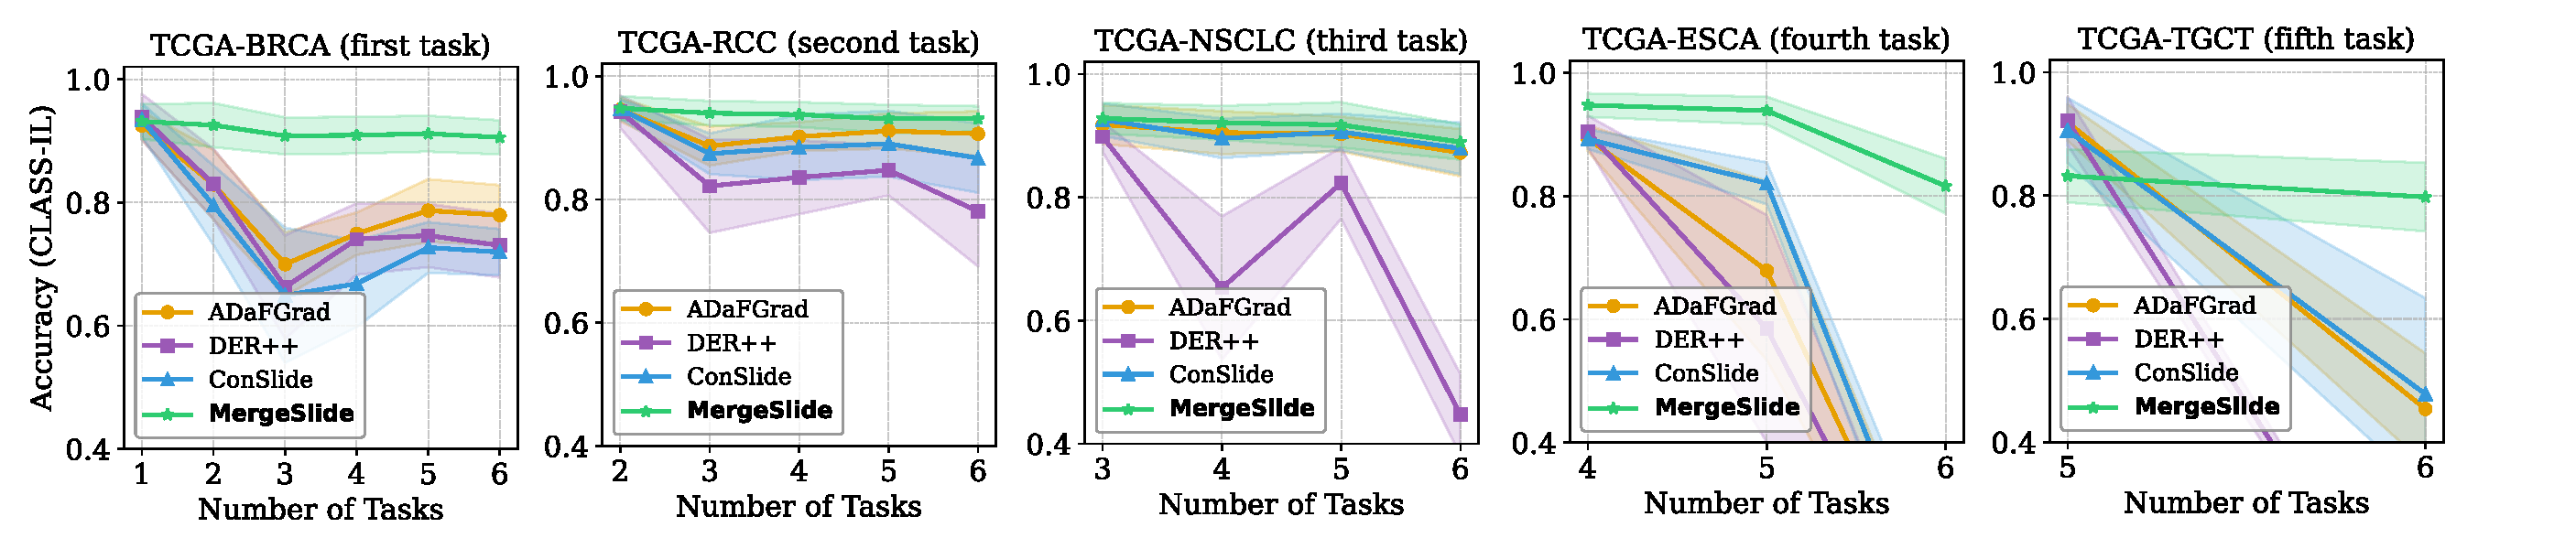
\includegraphics[width=1\textwidth]{forgetting_full.pdf}}
\caption{Performance drop comparisons across different methods as new tasks are added to the first five datasets: TCGA-BRCA, TCGA-RCC, TCGA-NSCLC, TCGA-ESCA, and TCGA-TGCT (sequence: \textcolor{blue}{B}$\rightarrow$\textcolor{blue}{R}$\rightarrow$\textcolor{blue}{N}$\rightarrow$\textcolor{red}{E}$\rightarrow$\textcolor{red}{T}$\rightarrow$\textcolor{red}{C}).}
\label{fig:forgetting} 
\end{figure*}

\begin{figure*}[!ht]
\centerline{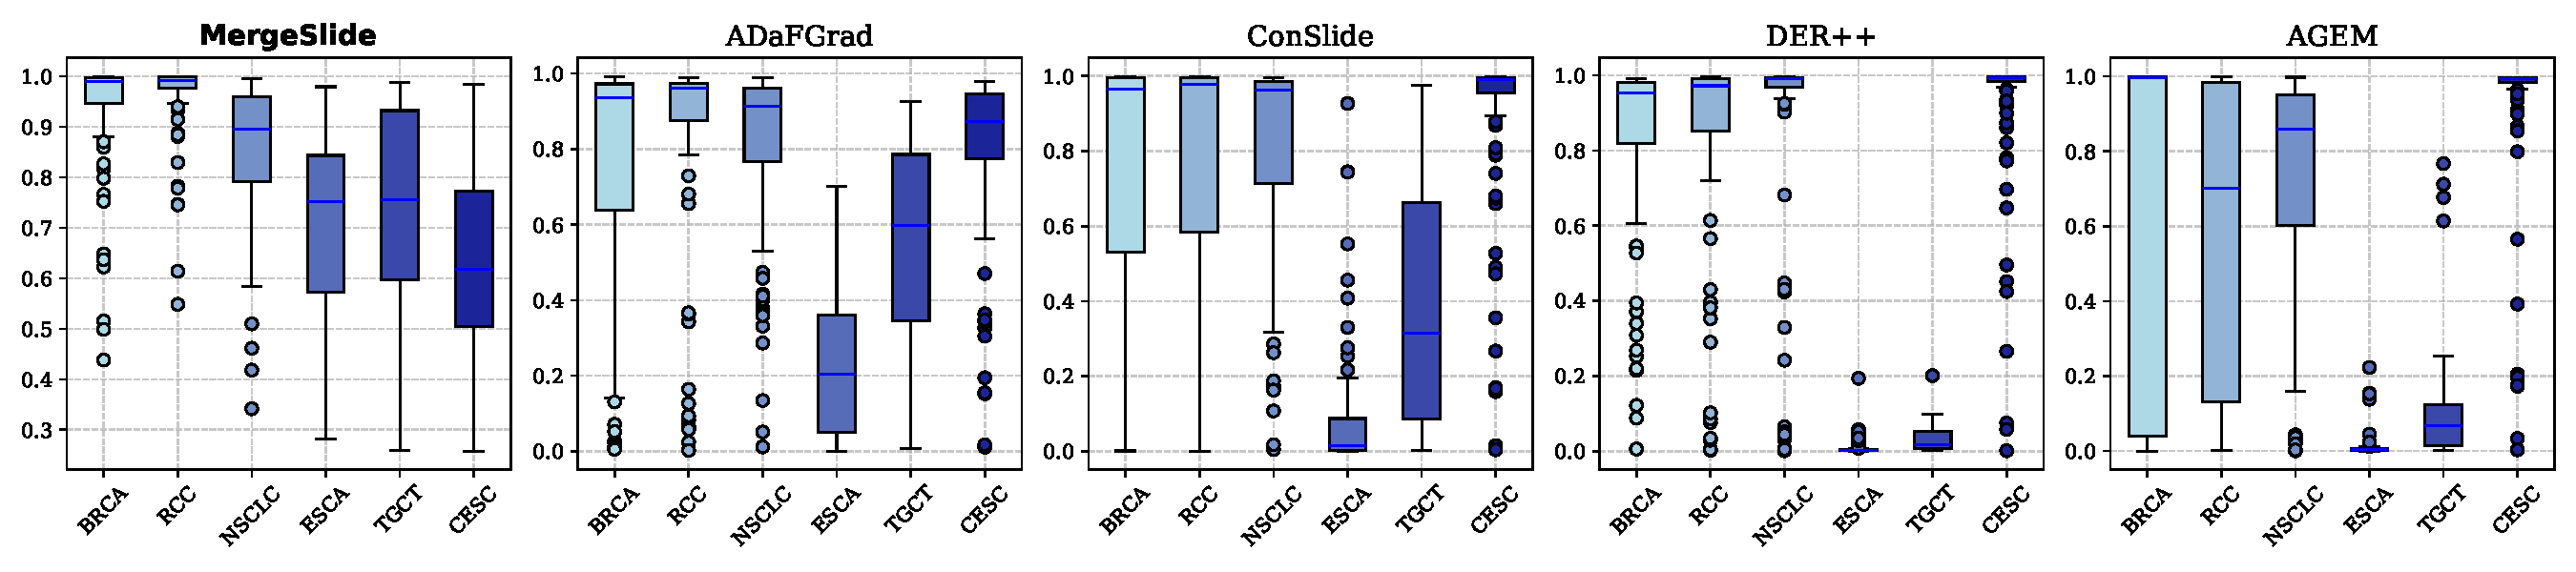
\includegraphics[width=1\textwidth]{logits.pdf}}
\caption{Comparison of average confidence scores for target cancer subtyping after training on the last task, TCGA-CESC (sequence: \textcolor{blue}{B}$\rightarrow$\textcolor{blue}{R}$\rightarrow$\textcolor{blue}{N}$\rightarrow$\textcolor{red}{E}$\rightarrow$\textcolor{red}{T}$\rightarrow$\textcolor{red}{C}).}
\label{fig:confidence_score} 
\end{figure*}

\subsection{What Happens When the MLP is Also Trained?} As described, only the backbone $f_{\mathcal{A}}$ is trained when a new task is added, in order to obtain the corresponding weight set $\theta_t$. We do not train the MLP as a classifier but instead use class-aware prompt embeddings $E^{\mathcal{C},t}$. Results in Tab.~\ref{tab:mlp} show that the MLP-free strategy not only avoids performance degradation but also slightly improves both Masked ACC and Mean ACC compared to trainable MLPs, regardless of whether \texttt{TCP} is used. The only exception is overall ACC when using \texttt{TCP}, which exhibits a very marginal decrease.

\begin{table}[!http]
\resizebox{\linewidth}{!}{\begin{tabular}{lcccc}
\toprule
\textbf{Method} & \textbf{MLP Setting} & \textbf{ACC}& \textbf{Masked ACC} & \textbf{Mean ACC}   \\ \midrule
\multirow{2}{*}{MergeSlide (naive)} & Trainable MLP& 78.613 ($\pm$1.710) & 93.534 ($\pm$0.831) & 90.075 ($\pm$1.145) \\
  & MLP-free (ours)  & \textbf{78.797 ($\pm$1.916)} & \textbf{93.617 ($\pm$1.098)} & \textbf{90.640 ($\pm$1.247)} \\ \midrule
\multirow{2}{*}{MergeSlide \texttt{w/ TCP}}  & Trainable MLP& \textbf{91.935 ($\pm$0.897)}  & 93.534 ($\pm$0.831)  & 92.137 ($\pm$1.287)  \\
  & MLP-free (ours)  & 91.914 ($\pm$0.980) & \textbf{93.617 ($\pm$1.098)} & \textbf{92.686 ($\pm$0.899)} \\ \bottomrule
\end{tabular}}
\caption{Comparison between two strategies for MLP: Trainable MLP and MLP-Free on the sequence of \textcolor{blue}{B}$\rightarrow$\textcolor{blue}{R}$\rightarrow$\textcolor{blue}{N}$\rightarrow$\textcolor{red}{E}$\rightarrow$\textcolor{red}{T}$\rightarrow$\textcolor{red}{C}.}
\label{tab:mlp}

\end{table}

\subsection{Task-wise Performance} We provide a task-wise performance comparison between the top three methods under the CLASS-IL and TASK-IL scenarios in Tabs. \ref{tab:class-il} and \ref{tab:task-il}, respectively, after training on the last task, i.e., TCGA-CESC. As a result, under the CLASS-IL scenario, MergeSlide still outperforms the others on five out of six tasks. Even without TCP, it achieves better performance than the others on four out of six tasks. However, we also observe that rehearsal-based methods tend to perform poorly on earlier tasks with limited WSIs, such as TCGA-ESCA and TCGA-TGCT. Indeed, after training on the final task (TCGA-CESC), the performance on this dataset becomes much higher compared to those with fewer samples. Nonetheless, MergeSlide maintains stable performance across tasks.

\begin{table}[H]
\centering
\resizebox{\linewidth}{!}{%
\begin{tabular}{lccc}
\toprule
\multicolumn{1}{l}{\textbf{Method}} & \textbf{BRCA} & \textbf{RCC} & \textbf{NSCLC} \\
\midrule
Zero-shot & 89.922 ($\pm$2.981) & 83.474 ($\pm$2.891) & 83.874 ($\pm$2.766) \\
DER++ \cite{derpp} ($|\mathcal{B}_r|=30$) & 73.026 ($\pm$5.194) & 78.055 ($\pm$8.936) & 44.730 ($\pm$6.570) \\
ConSlide \cite{huang2023conslide} ($|\mathcal{B}_r|=30$) & 71.940 ($\pm$3.949) & 86.700 ($\pm$5.921) & 87.933 ($\pm$4.409) \\
ADaFGrad \cite{adafgrad} ($|\mathcal{B}_r|=30$) & 77.938 ($\pm$4.871) & 90.647 ($\pm$3.636) & 87.252 ($\pm$3.843) \\ \midrule
\textbf{MergeSlide} & \textbf{91.045 ($\pm$3.047)} & \underline{93.183 ($\pm$2.019)} & \underline{89.331 ($\pm$3.089)} \\
\textbf{MergeSlide w/ \texttt{TCP}} & \underline{90.784 ($\pm$3.311)} & \textbf{93.418 ($\pm$2.351)} & \textbf{93.657 ($\pm$2.633)} \\
\bottomrule
\end{tabular}}
\vspace{0.3cm}
\resizebox{\linewidth}{!}{%
\begin{tabular}{lccc}
\toprule
\multicolumn{1}{l}{\textbf{Method}} & \textbf{ESCA} & \textbf{TGCT} & \textbf{CESC} \\
\midrule
Zero-shot & 62.388 ($\pm$3.704) & \underline{79.771 ($\pm$5.316)} & 17.578 ($\pm$2.928) \\
DER++ \cite{derpp} ($|\mathcal{B}_r|=30$) & 2.836 ($\pm$2.707) & 0.526 ($\pm$1.053) & \underline{93.516 ($\pm$1.310)} \\
ConSlide \cite{huang2023conslide} ($|\mathcal{B}_r|=30$) & 8.657 ($\pm$6.814) & 45.371 ($\pm$9.516) & \textbf{93.531 ($\pm$2.209)} \\
ADaFGrad \cite{adafgrad} ($|\mathcal{B}_r|=30$) & 6.269 ($\pm$5.247) & 47.787 ($\pm$15.559) & 93.594 ($\pm$1.148) \\ \midrule
\textbf{MergeSlide} & 81.940 ($\pm$3.802) & 79.507 ($\pm$5.541) & 52.266 ($\pm$7.562) \\
\textbf{MergeSlide w/ \texttt{TCP}} & \textbf{94.925 ($\pm$2.331)} & \textbf{81.343 ($\pm$5.616)} & 92.031 ($\pm$1.389) \\
\bottomrule
\end{tabular}}
\caption{Task-wise performances on stream of datasets \textcolor{blue}{B}$\rightarrow$\textcolor{blue}{R}$\rightarrow$\textcolor{blue}{N}$\rightarrow$\textcolor{red}{E}$\rightarrow$\textcolor{red}{T}$\rightarrow$\textcolor{red}{C} under CLASS-IL scenario.}
\label{tab:class-il}
\end{table}

\begin{table}[H]
\centering
\resizebox{\linewidth}{!}{%
\begin{tabular}{lccc}
\toprule
\multicolumn{1}{l}{\textbf{Method}} & \textbf{BRCA} & \textbf{RCC} & \textbf{NSCLC} \\
\midrule
Zero-shot & 91.643 ($\pm$2.969) & 83.591 ($\pm$2.914) & 89.917 ($\pm$1.857) \\
DER++ \cite{derpp} ($|\mathcal{B}_r|=30$) & 84.783 ($\pm$5.802) & 89.113 ($\pm$5.243) & 88.952 ($\pm$2.989) \\
ConSlide \cite{huang2023conslide} ($|\mathcal{B}_r|=30$) & 87.604 ($\pm$4.920) & 92.574 ($\pm$4.466) & \underline{92.265 ($\pm$2.503)} \\
ADaFGrad \cite{adafgrad} ($|\mathcal{B}_r|=30$) & 86.582 ($\pm$4.129) & \textbf{93.652 ($\pm$2.434)} & 91.458 ($\pm$2.817) \\ \midrule
\textbf{MergeSlide} & \textbf{93.359 ($\pm$3.353)} & \underline{93.645 ($\pm$2.100)} & \textbf{92.939 ($\pm$2.539)} \\
\bottomrule
\end{tabular}}
\vspace{0.3cm}
\resizebox{\linewidth}{!}{%
\begin{tabular}{lccc}
\toprule
\multicolumn{1}{l}{\textbf{Method}} & \textbf{ESCA} & \textbf{TGCT} & \textbf{CESC} \\
\midrule
Zero-shot & 88.060 ($\pm$2.111) & 81.862 ($\pm$5.855) & \textbf{95.859 ($\pm$1.108)} \\
DER++ \cite{derpp} ($|\mathcal{B}_r|=30$) & 87.185 ($\pm$3.379) & \textbf{92.153 ($\pm$3.806)} & 93.913 ($\pm$1.201) \\
ConSlide \cite{huang2023conslide} ($|\mathcal{B}_r|=30$) & 87.797 ($\pm$4.649) & \underline{91.641 ($\pm$7.755)} & 94.099 ($\pm$2.119) \\
ADaFGrad \cite{adafgrad} ($|\mathcal{B}_r|=30$) & 88.152 ($\pm$3.832) & 90.799 ($\pm$7.266) & \underline{94.362 ($\pm$1.164)} \\ \midrule
\textbf{MergeSlide} & \textbf{95.075 ($\pm$1.772)} & 91.066 ($\pm$2.433) & 94.297 ($\pm$1.443) \\
\bottomrule
\end{tabular}}
\caption{Task-wise performances on stream of datasets \textcolor{blue}{B}$\rightarrow$\textcolor{blue}{R}$\rightarrow$\textcolor{blue}{N}$\rightarrow$\textcolor{red}{E}$\rightarrow$\textcolor{red}{T}$\rightarrow$\textcolor{red}{C} under TASK-IL scenario.}
\label{tab:task-il}
\end{table}

\subsection{Task Addition} Final accuracy after merging weights reflects the end performance; however, performance during the addition of new tasks should also be examined to ensure stability. The comparison of CLASS-IL ACC for MergeSlide against other methods is reported in Tab.~\ref{tab:sequence}, where the number of accumulated tasks $T \in \{2, 3, 4, 5\}$ is evaluated. The results show that some methods exhibit unstable performance \textit{while MergeSlide demonstrates consistent performances as the number of tasks increases.} $\sigma < 1\%$ further confirms the stability. We further compare performance drops on the two earliest tasks, TCGA-BRCA and TCGA-RCC, across top methods and MergeSlide without \texttt{TCP} (Fig.~\ref{fig:forgetting}). MergeSlide maintains stable performance as new tasks arrive, while others show significant and moderate drops on TCGA-BRCA and TCGA-RCC, respectively.

\begin{table}[H]
\centering
\resizebox{\linewidth}{!}{%
\begin{tabular}{lccccc}
\toprule
\multicolumn{1}{l}{} & \multicolumn{4}{c}{Number of increasing tasks} & \\
\cmidrule(lr){2-5}
\multicolumn{1}{l}{Method} & \textit{T=2} & \textit{T=3} & \textit{T=4} & \textit{T=5} & $\sigma$ \\
\midrule
ER-ACE & 90.045 ($\pm$1.968) & 81.210 ($\pm$2.793) & 79.297 ($\pm$4.234) & 74.849 ($\pm$5.461) & 5.525 \\
AGEM   & 84.839 ($\pm$9.500) & 70.843 ($\pm$4.327) & 75.236 ($\pm$6.225) & 75.169 ($\pm$4.972) & 5.121 \\
DER++  & \underline{92.244 ($\pm$3.177)} & \underline{86.693 ($\pm$2.215)} & \underline{88.104 ($\pm$1.323)} & 82.307 ($\pm$2.946) & 3.549 \\
ConSlide   & 86.733 ($\pm$2.228) & 80.643 ($\pm$3.226) & 83.929 ($\pm$1.968) & 85.257 ($\pm$2.068) & 2.250 \\
ADaFGrad   & 90.945 ($\pm$3.214) & 86.002 ($\pm$2.225) & 87.382 ($\pm$1.908) & \underline{85.252 ($\pm$2.271)} & 2.187 \\ \midrule
\textbf{MergeSlide} & \textbf{92.907 ($\pm$1.337)} & \textbf{92.571 ($\pm$0.713)} & \textbf{93.309 ($\pm$0.493)} & \textbf{92.345 ($\pm$0.990)} & \textbf{0.364} \\
\bottomrule
\end{tabular}}
\caption{Closer look at MergeSlide compared to other continual learning methods as the number of tasks increases on the sequence of \textcolor{blue}{B}$\rightarrow$\textcolor{blue}{R}$\rightarrow$\textcolor{blue}{N}$\rightarrow$\textcolor{red}{E}$\rightarrow$\textcolor{red}{T}$\rightarrow$\textcolor{red}{C} (Metric: CLASS-IL ACC). $\sigma$ shows the standard deviation of results across $T \in \{2, 3, 4, 5\}$.}
\label{tab:sequence}
\end{table}

\subsection{Sensitivity of number of patches $K$}

{To further examine the sensitivity of the sampling patch number $K$, we report the bACC of MergeSlide under both CLASS-IL and TASK-IL settings for $K \in {50, 100, 200, 300, 400}$ in Tab. \ref{tab:sensitivity}. In the CLASS-IL scenario, results without TCP remain stable, while with TCP the performance gap between $K=50$ and $K=400$ is only $4.997\%$. In the TASK-IL scenario, performance is also stable across different $K$ values. Notably, even the lowest setting ($K=50$) still outperforms all comparative baselines.}

\begin{table}[!h]
\resizebox{\linewidth}{!}{{\begin{tabular}{clll}
\toprule
\multicolumn{1}{c}{\multirow{2}{*}{\textbf{$K$}}} & \multicolumn{2}{c}{\textbf{\begin{tabular}[c]{@{}c@{}}bACC \\ (CLASS-IL)\end{tabular}}}                    & \multicolumn{1}{c}{\textbf{\begin{tabular}[c]{@{}c@{}}Masked bACC\\ (TASK-IL)\end{tabular}}} \\ \cmidrule{2-4}
\multicolumn{1}{c}{}         & \multicolumn{1}{c}{\textbf{\begin{tabular}[c]{@{}c@{}}MergeSlide\\ \texttt{w/o TCP}\end{tabular}}} & \multicolumn{1}{c}{\textbf{\begin{tabular}[c]{@{}c@{}}MergeSlide\\ \texttt{w/ TCP}\end{tabular}}} & \multicolumn{1}{c}{\textbf{MergeSlide}}    \\ \midrule
50 & 78.810 ($\pm$1.942) & 82.932 ($\pm$1.802)& 90.935 ($\pm$1.870)    \\
100& 80.167 ($\pm$1.752) & 84.284 ($\pm$2.478)& 91.610 ($\pm$1.535)    \\
200& 80.078 ($\pm$1.952) & 86.269 ($\pm$1.975)& 91.761 ($\pm$1.907)    \\
300& 79.849 ($\pm$1.944) & 87.416 ($\pm$2.015)& 92.083 ($\pm$1.514)    \\
400& \textbf{80.668 ($\pm$1.860)} & \textbf{87.929 ($\pm$2.110)}& \textbf{92.087 ($\pm$1.740)}    \\ \bottomrule
\end{tabular}}}
\caption{{Sensitivity of $K$ sampling patches under the CLASS-IL and TASK-IL scenarios on \textcolor{blue}{B}$\rightarrow$\textcolor{blue}{R}$\rightarrow$\textcolor{blue}{N}$\rightarrow$\textcolor{red}{E}$\rightarrow$\textcolor{red}{T}$\rightarrow$\textcolor{red}{C}.}}
\label{tab:sensitivity}
\end{table}

% \section{Limitations}\label{sec:limitations}

% We also discuss the limitations of MergeSlide. Despite its success, the continual merge strategy still exhibits some variance with respect to the order of task sequences (although small), and it depends on the pre-trained model $f_{\mathcal{A}}$ for base knowledge. Furthermore, as it is MLP-free and adaptive, class-aware prompts must be carefully designed when new tasks are introduced to ensure good performance. Nevertheless, we believe MergeSlide remains an efficient framework for continual learning on WSIs, where data for each task may be very limited and subject to privacy constraints.

{\small
\bibliographystyle{ieee_fullname}
\bibliography{egbib}
}

\end{document}